\documentclass[a4paper]{article}
\usepackage[utf8]{inputenc}
\usepackage[T1]{fontenc}

\usepackage[backend=biber,sorting=none]{biblatex}
\addbibresource{references.bib}

\usepackage{amsmath}
\usepackage{appendix}
\usepackage{graphicx}
\usepackage{hyperref}
\usepackage{placeins}
\usepackage{subcaption}

\title{PAP328 project work: proportional counter}
\author{Mika Mäki}

% TODO add date when the report was handed in


\begin{document}

\maketitle

\section*{Abstract}
In this project we assembled a gas-based proportional counter for X-ray and $\gamma$-ray detection.
The detector consists of a cylindrical cathode, for which we used a beverage can, and a thin anode wire along its center.
When high voltage is applied between the cathode and the anode and incoming high-energy radiation ionizes the gas inside, the resulting electrons drift towards the anode wire.
Close to the wire the field strength is high enough for avalanche formation, and the electrons are multiplied, resulting in an electrical pulse that can be detected with electronics.

The system was tested with Fe-55 and Am-241 sources, and a multichannel analyzer was used to collect the emission spectra, which were then analyzed with self-developed software.
This setup demonstrated sufficient resolution to distinguish the TODO peaks.

TODO add main results here.

The detector was also tested with a self-built pre-amplifier.
However, these results were inconclusive due to unexpected degradation of the detector.
These measurements are discussed in the appendix \ref{pre_amp}.

\tableofcontents


\section{Introduction}
What are radiation detectors?
Basics of proportional counters.

Context for the usages!


\section{Theory}
Formulas here and only here

\subsection{The proportional counter}
The detector.
Electric field, gas composition, quenching, multiplication, different regions.
Theoretical predictions on accuracy?

TODO refer to the article "A gaseous proportional counter built from a conventional aluminum beverage can"

\subsection{Error analysis methods}
Error propagation formulas etc.

\subsection{Read-out electronics}



\section{Experimental set-up}
Self-built detector etc.
Answer the questions on page 5 of the instructions!


\subsection{Detector assembly}
Detector structure and construction steps

The top of the can was removed.
Holes.

\begin{figure}[ht!]
\centering
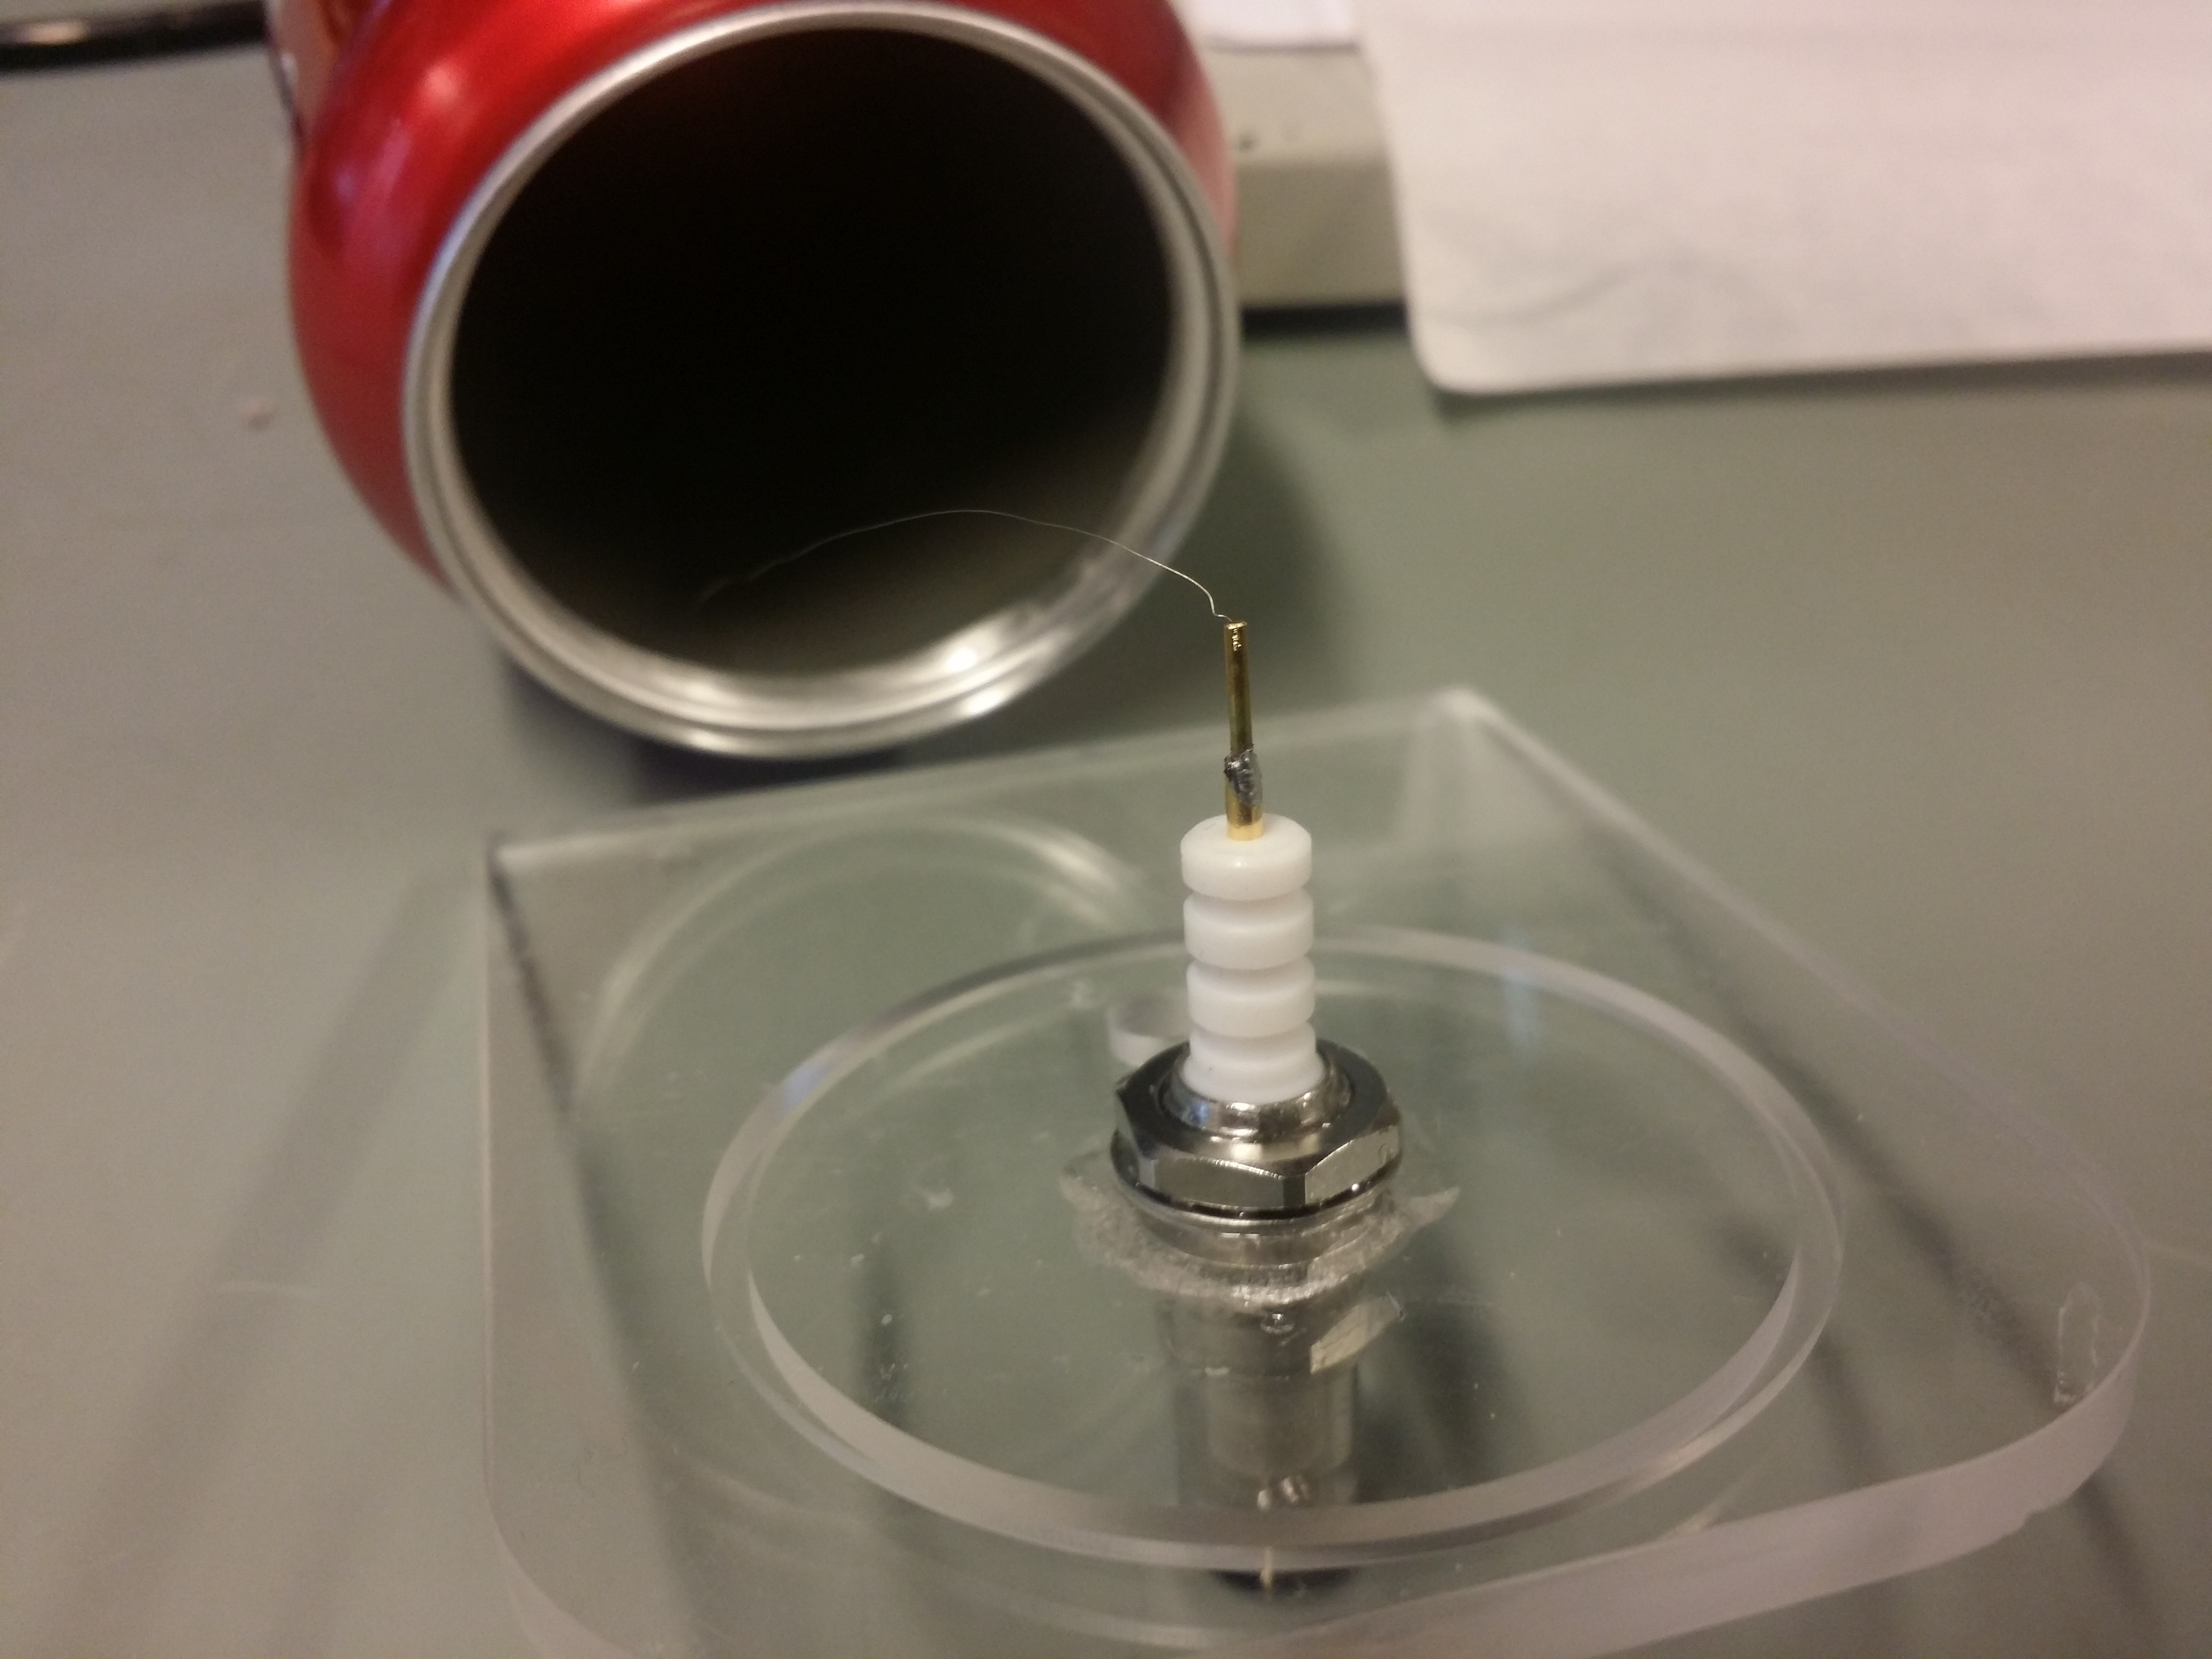
\includegraphics[width=\textwidth]{fig/IMG_20201117_121044.jpg}
\caption{The anode wire is soldered to the connector}
\end{figure}

\begin{figure}[ht!]
\centering
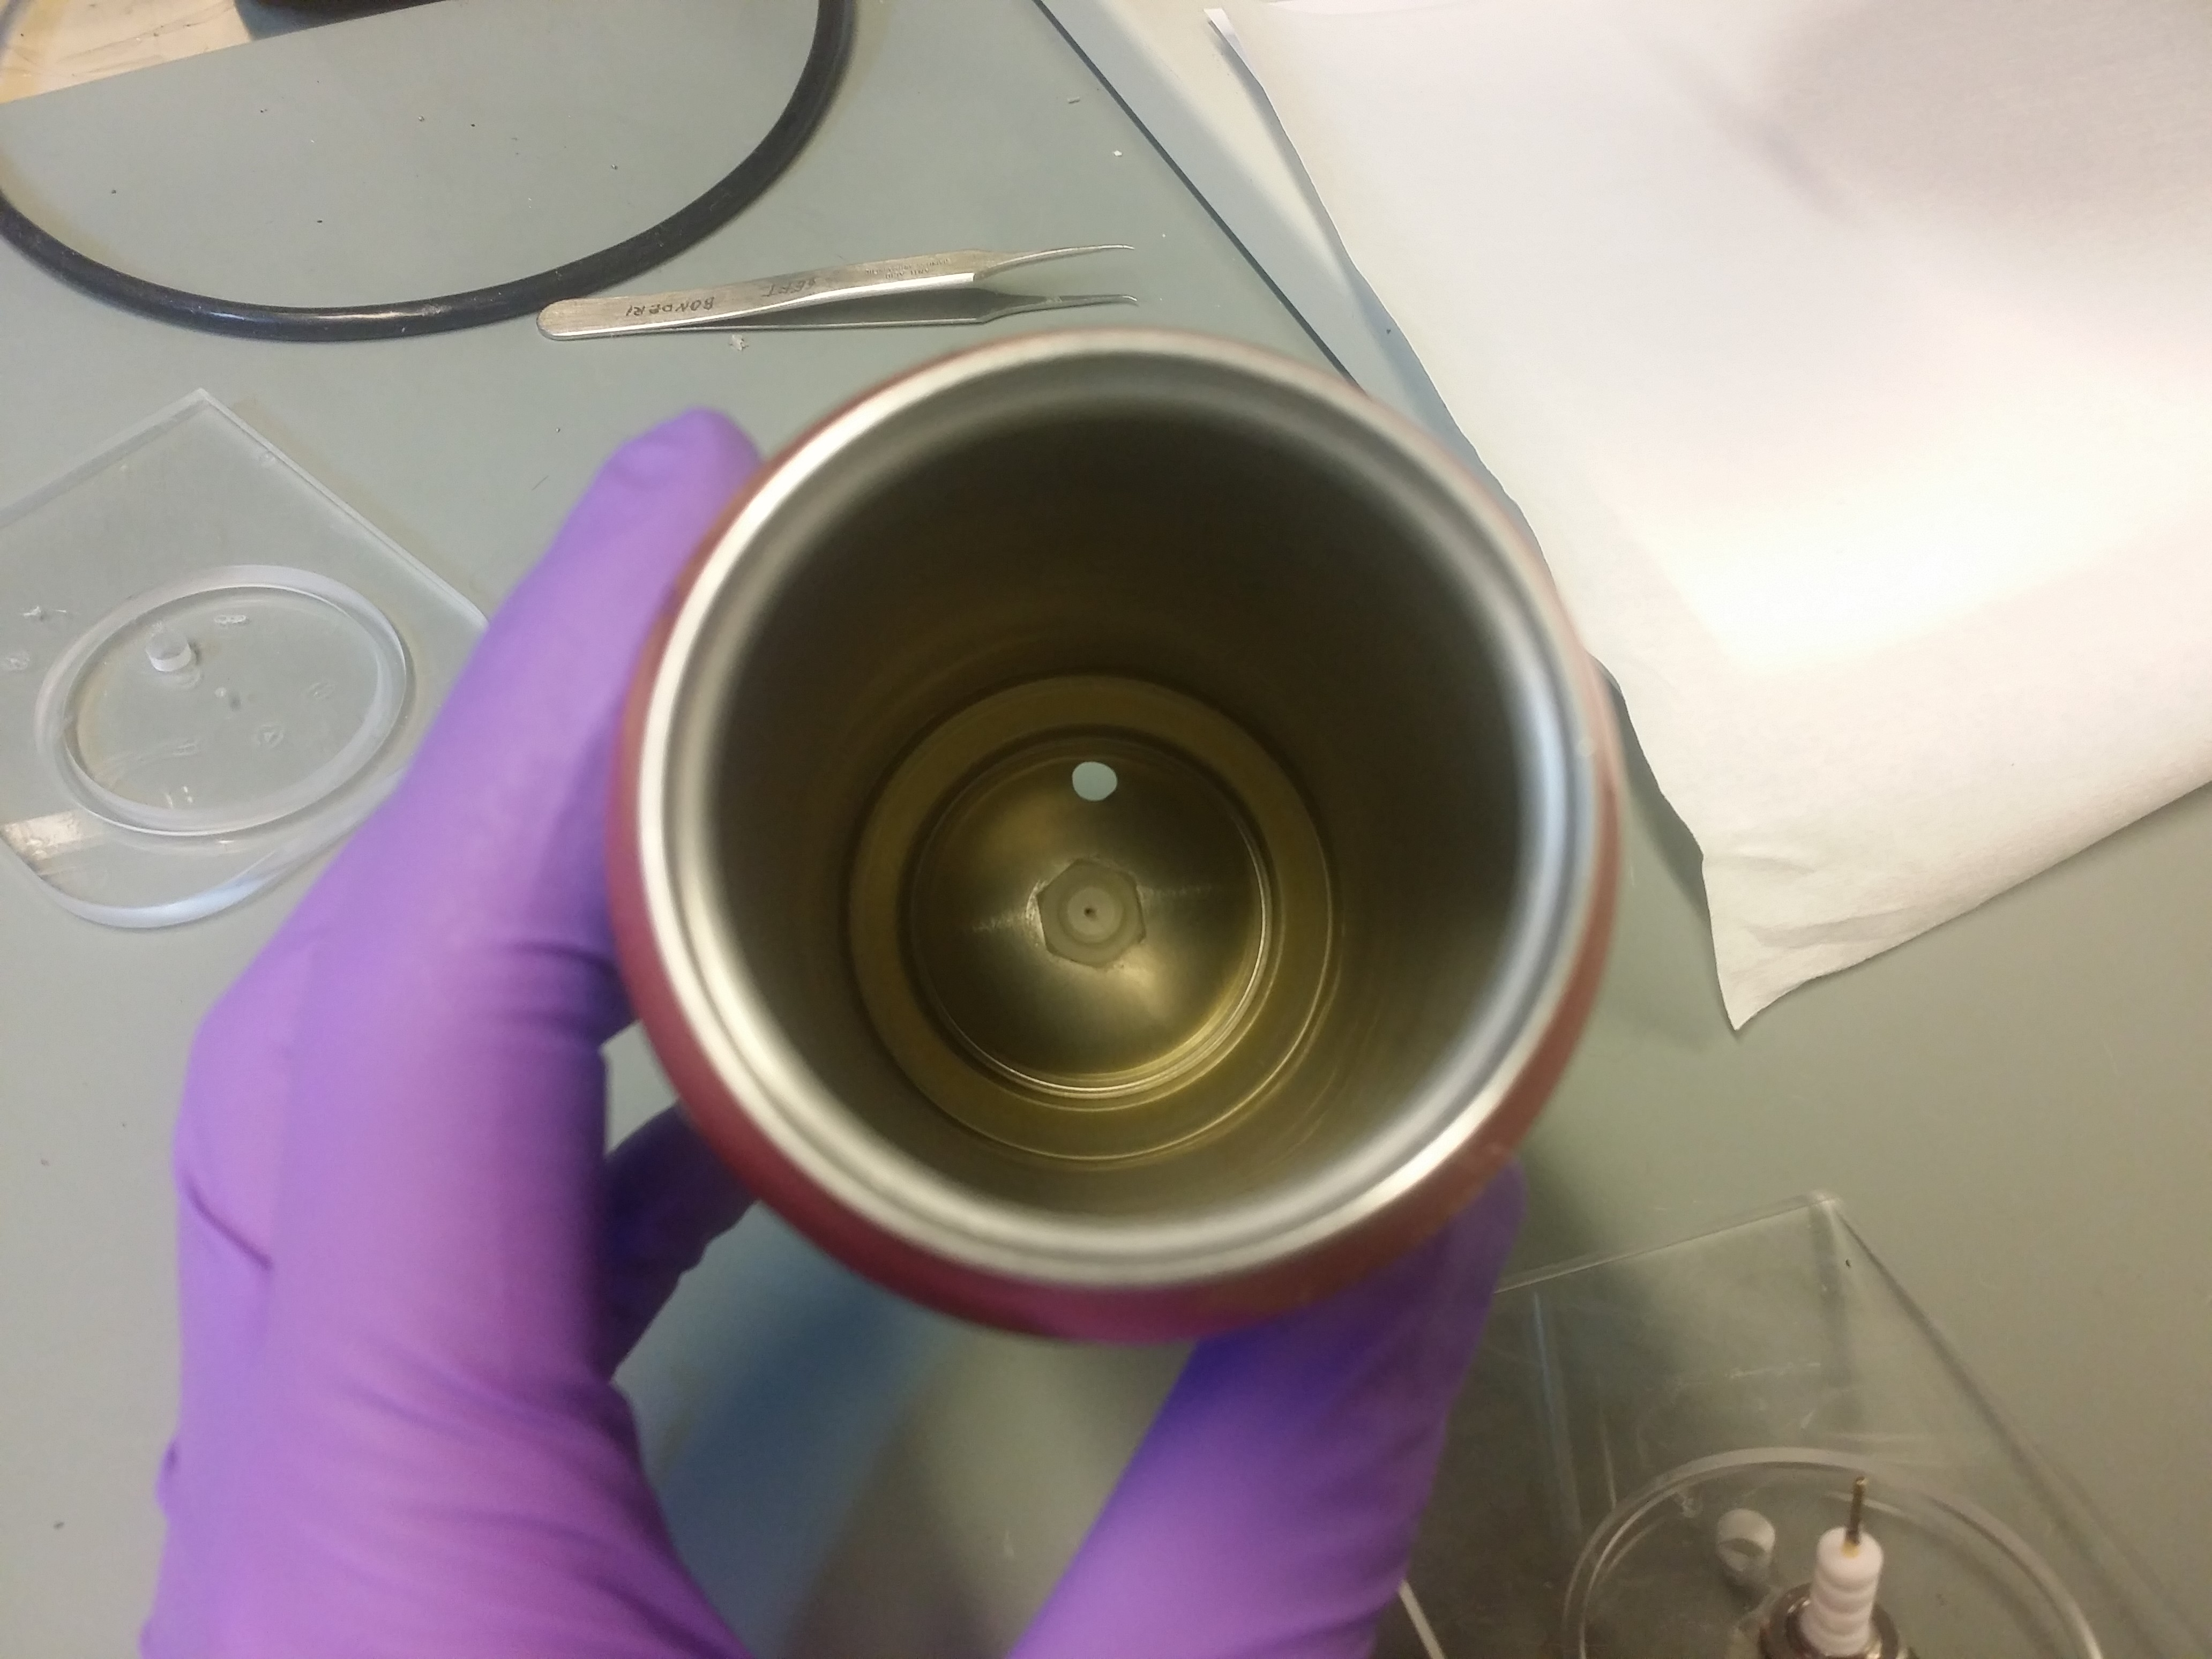
\includegraphics[width=\textwidth]{fig/IMG_20201123_103327.jpg}
\caption{A brass tube within a plastic screw serves as the other end of the anode wire}
\end{figure}

\begin{figure}[ht!]
\centering
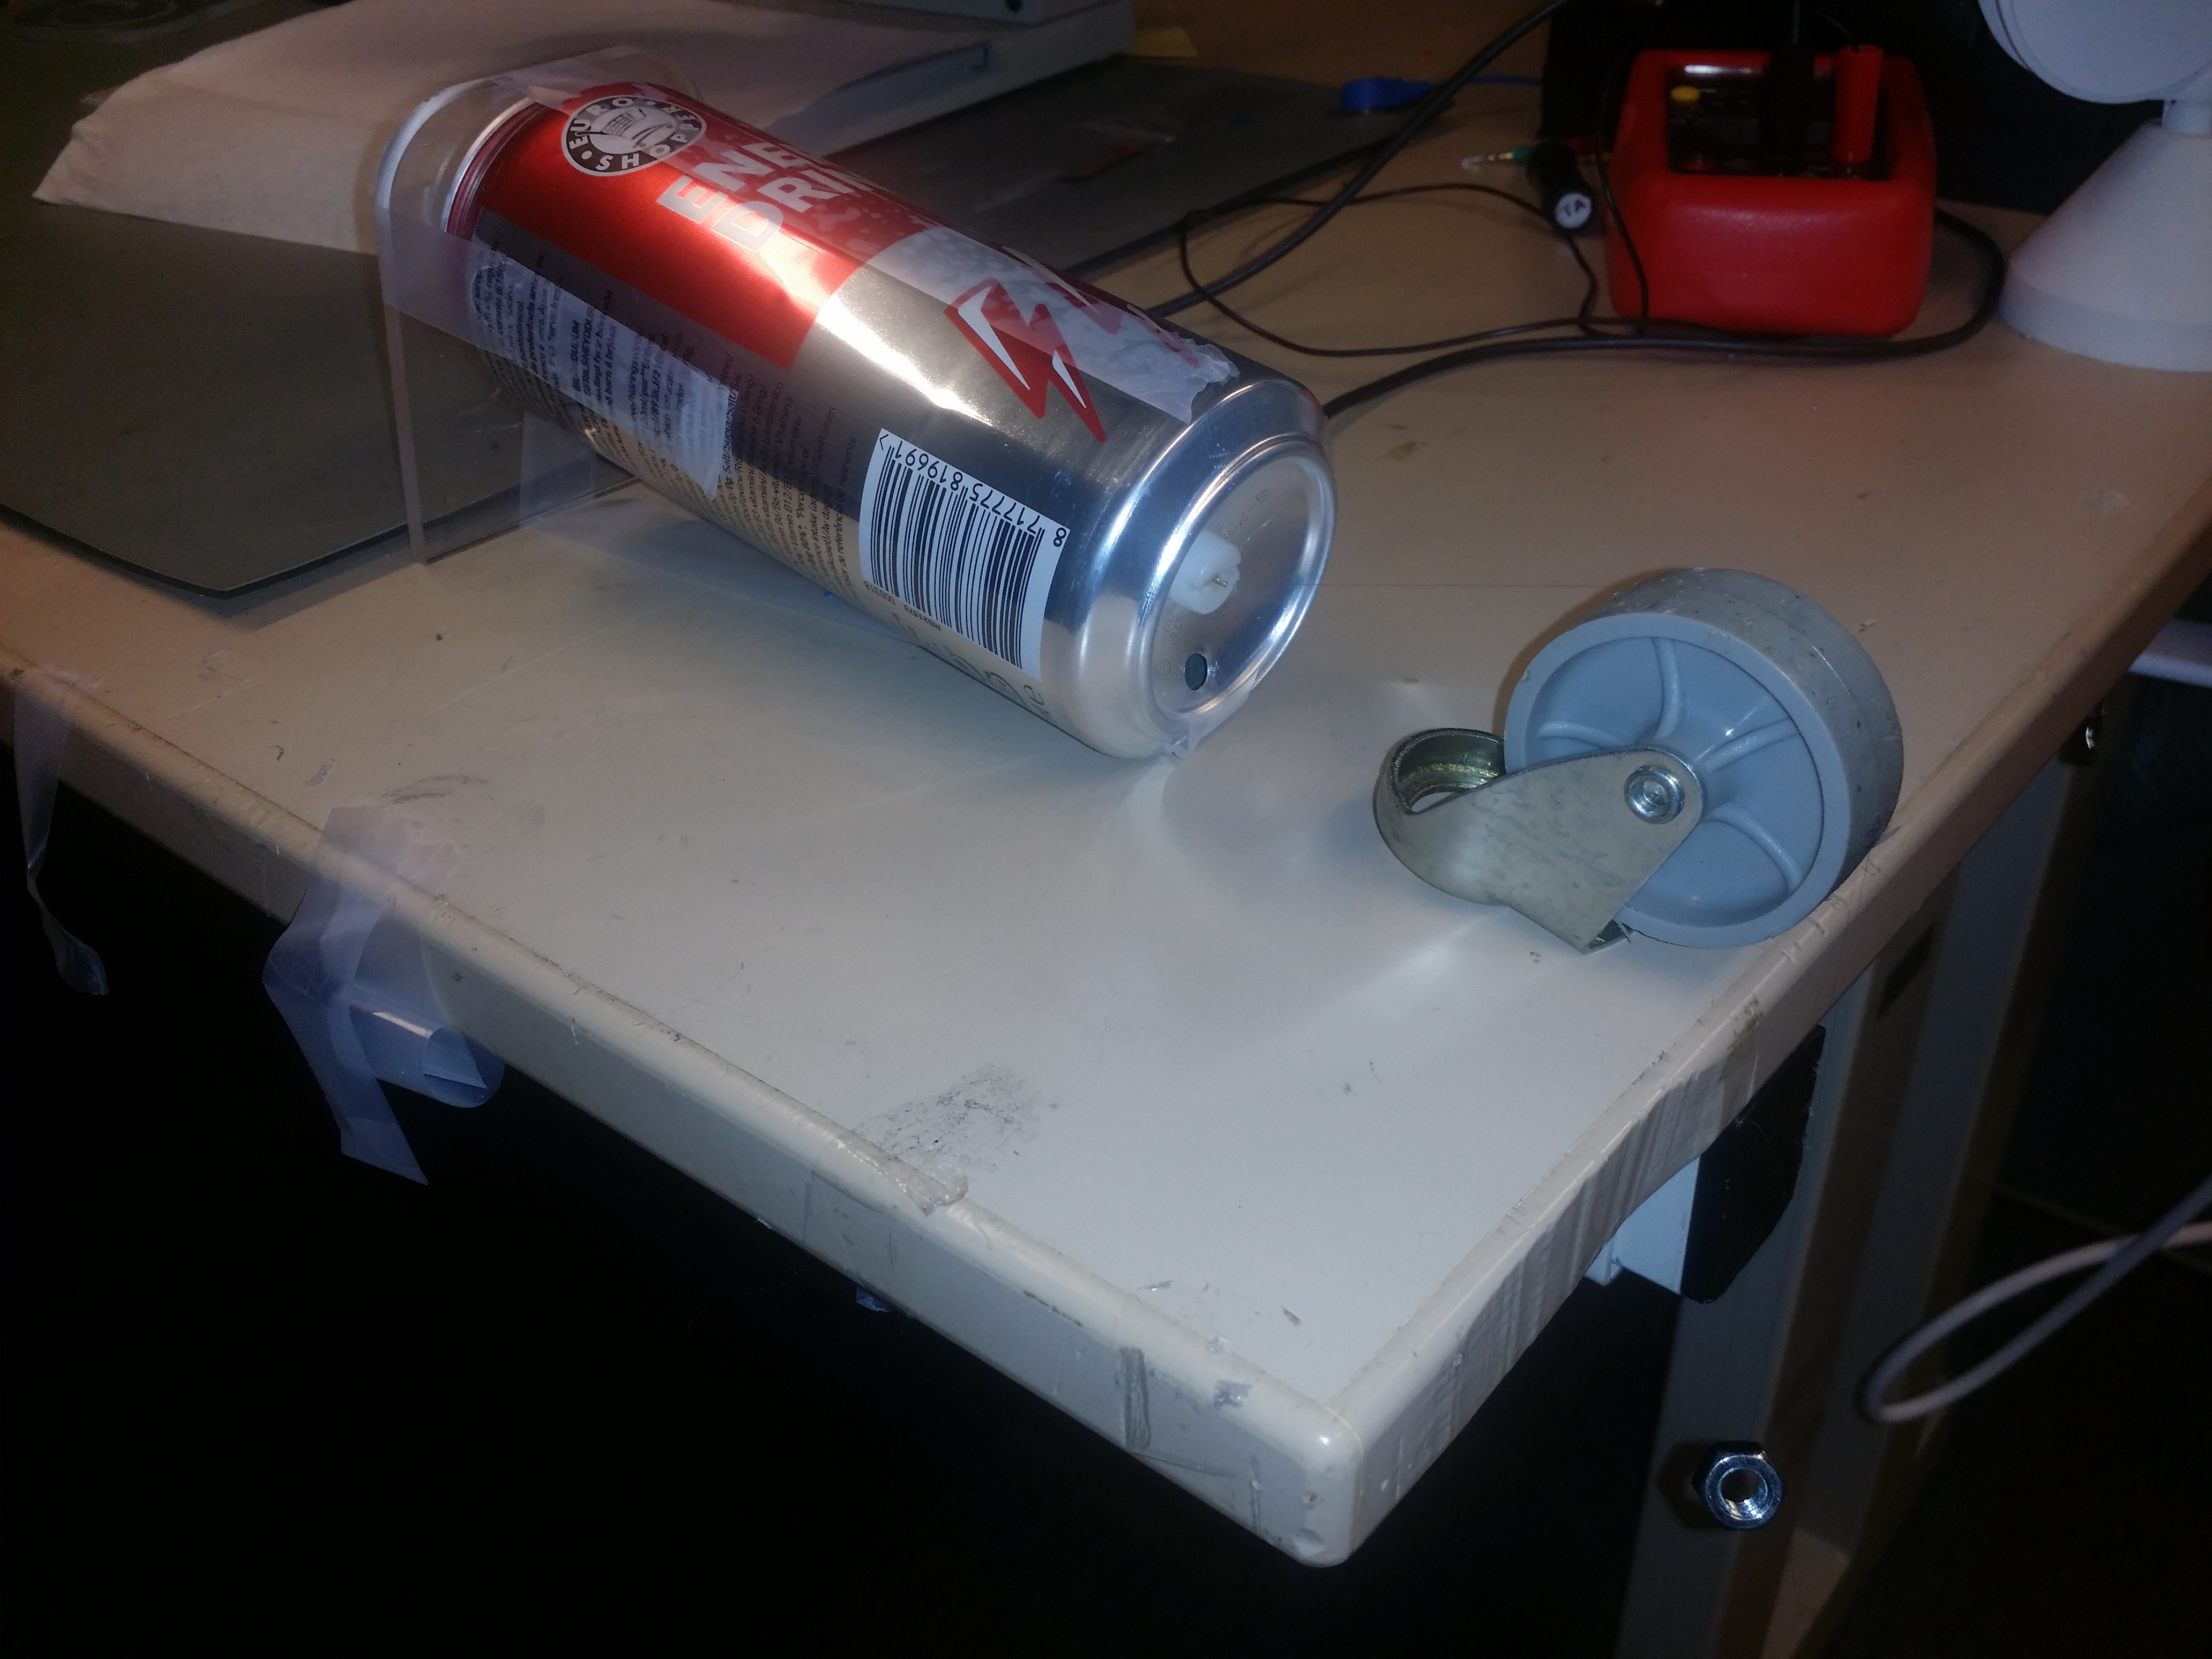
\includegraphics[width=\textwidth]{fig/IMG_20201123_104201.jpg}
\caption{Setup for soldering the anode (TODO CHECK) wire}
\end{figure}


\FloatBarrier
\subsection{Calibration}
The electronics have to be calibrated with an external pulser

\begin{figure}[ht!]
\centering
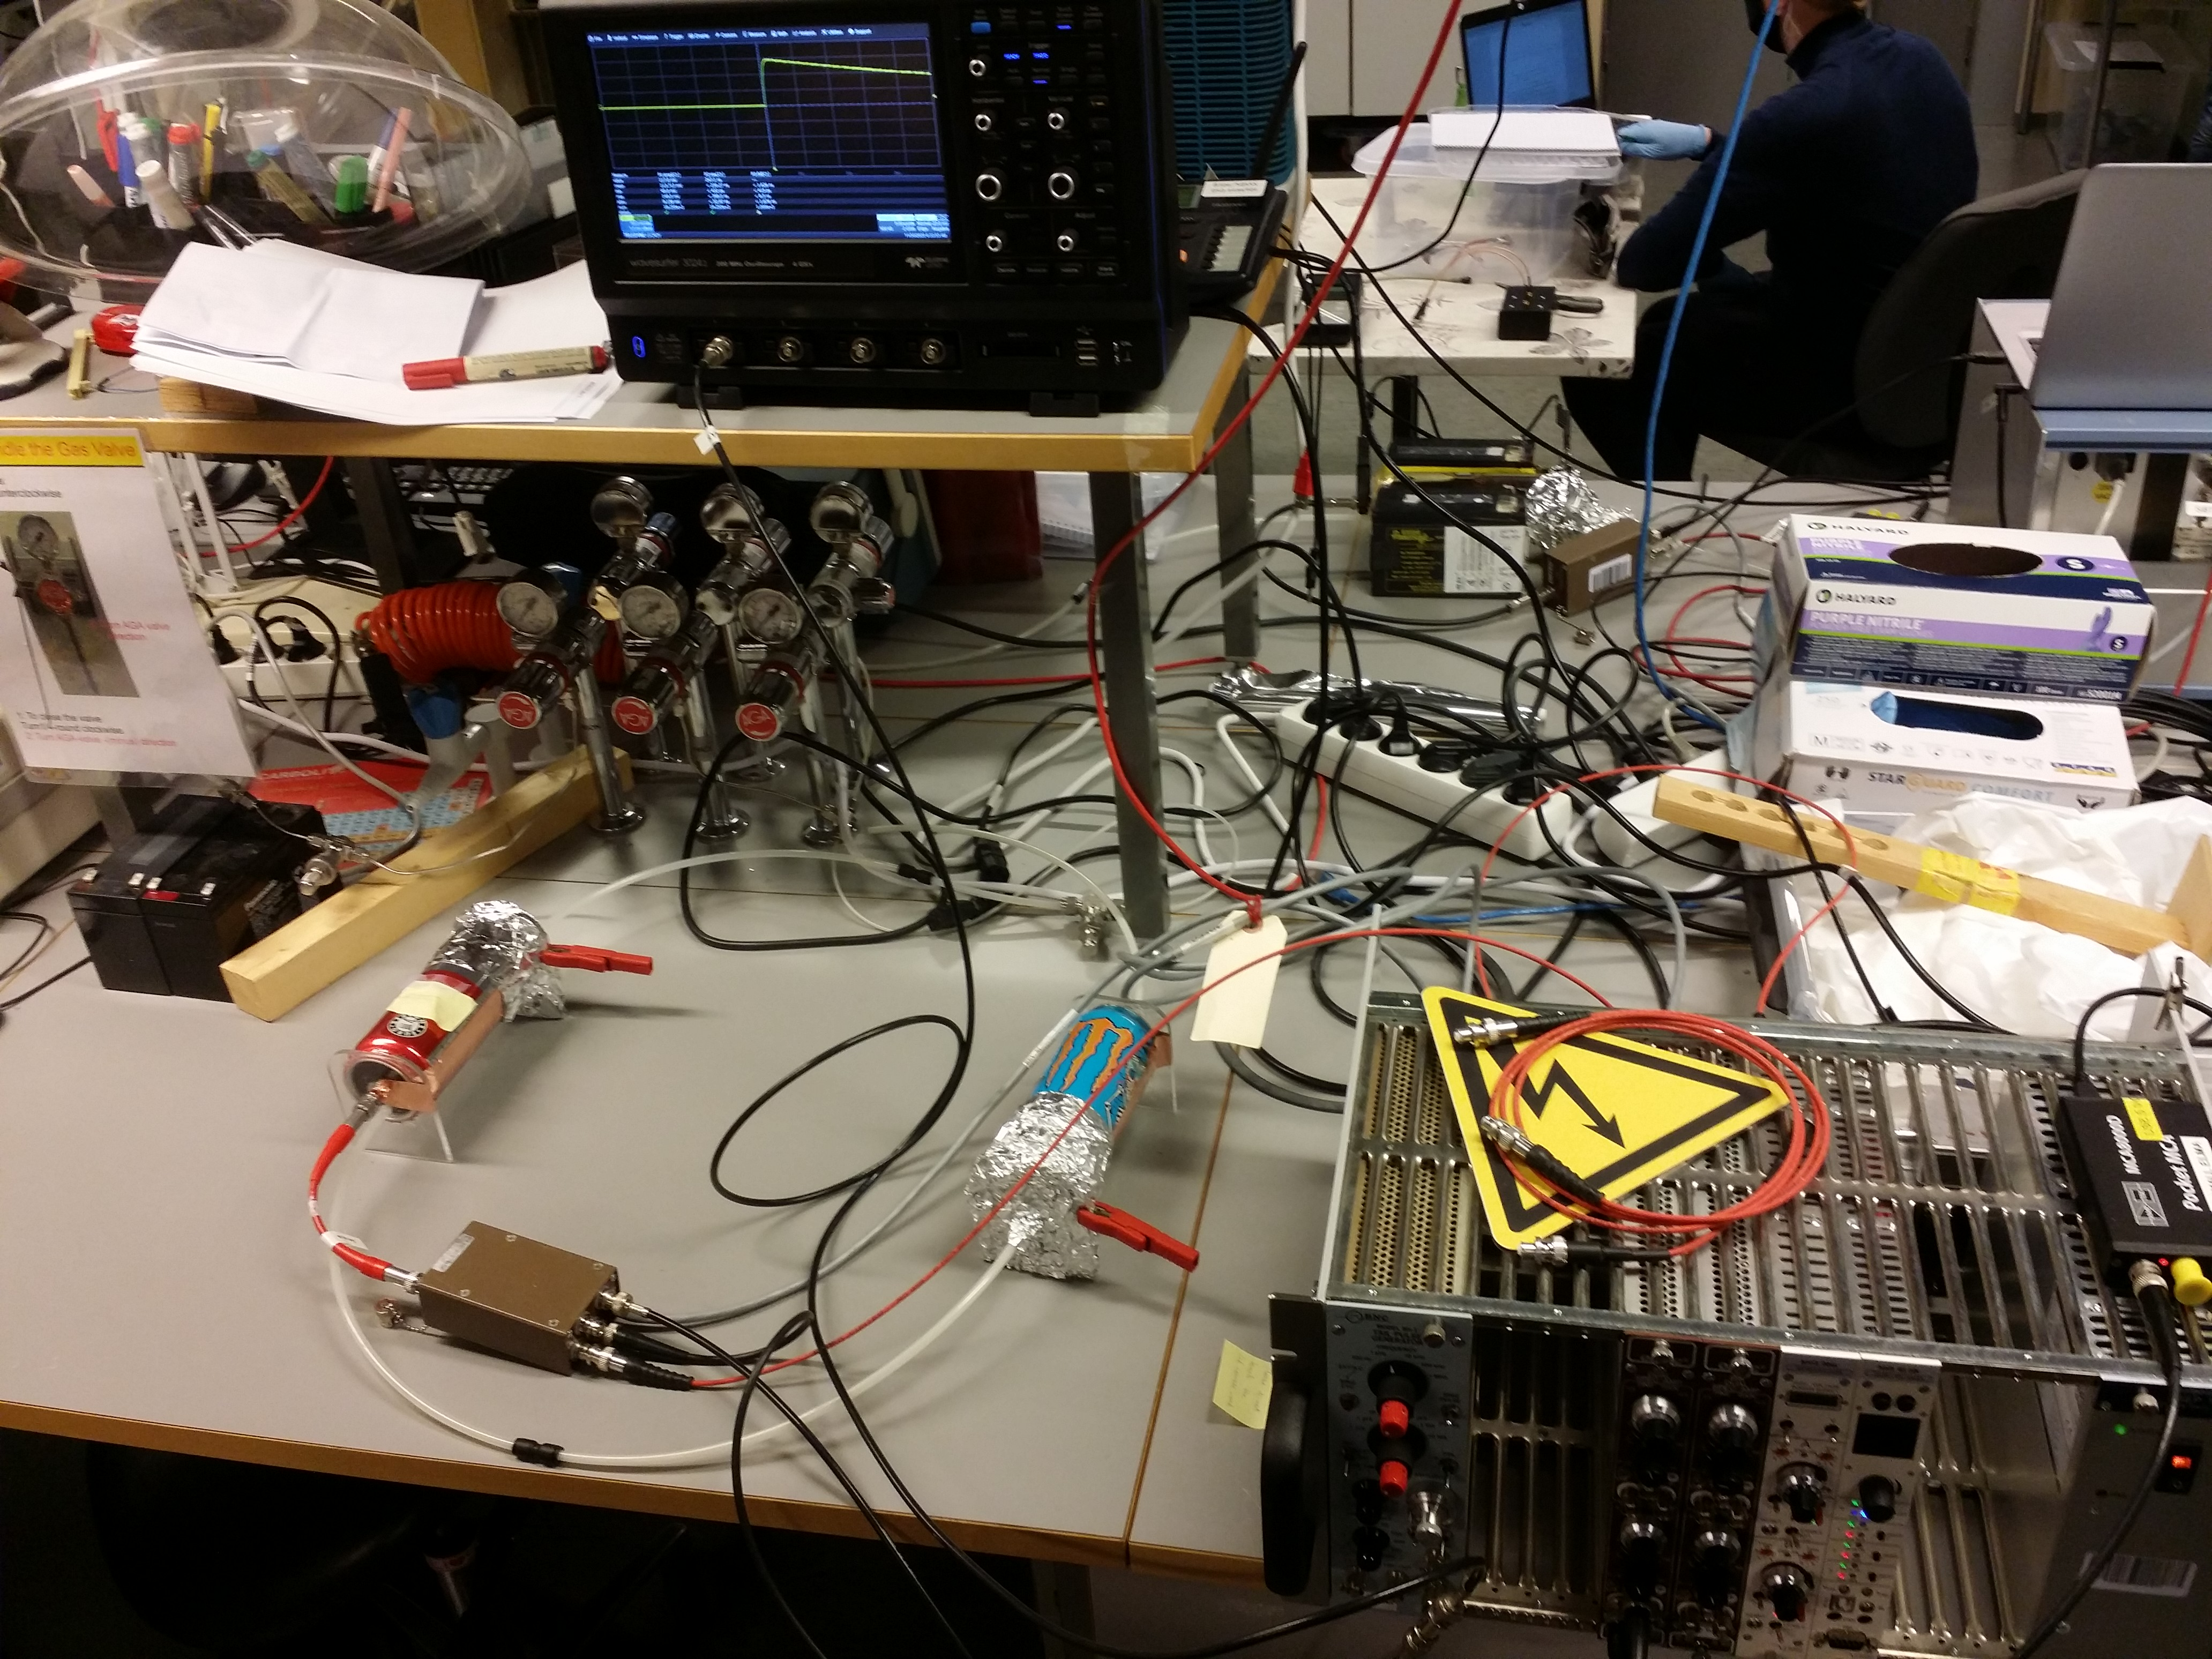
\includegraphics[width=\textwidth]{fig/IMG_20201130_135000.jpg}
\caption{Setup for testing with an external pulser}
\end{figure}


\FloatBarrier
\subsection{Testing}

\begin{figure}[ht!]
\centering
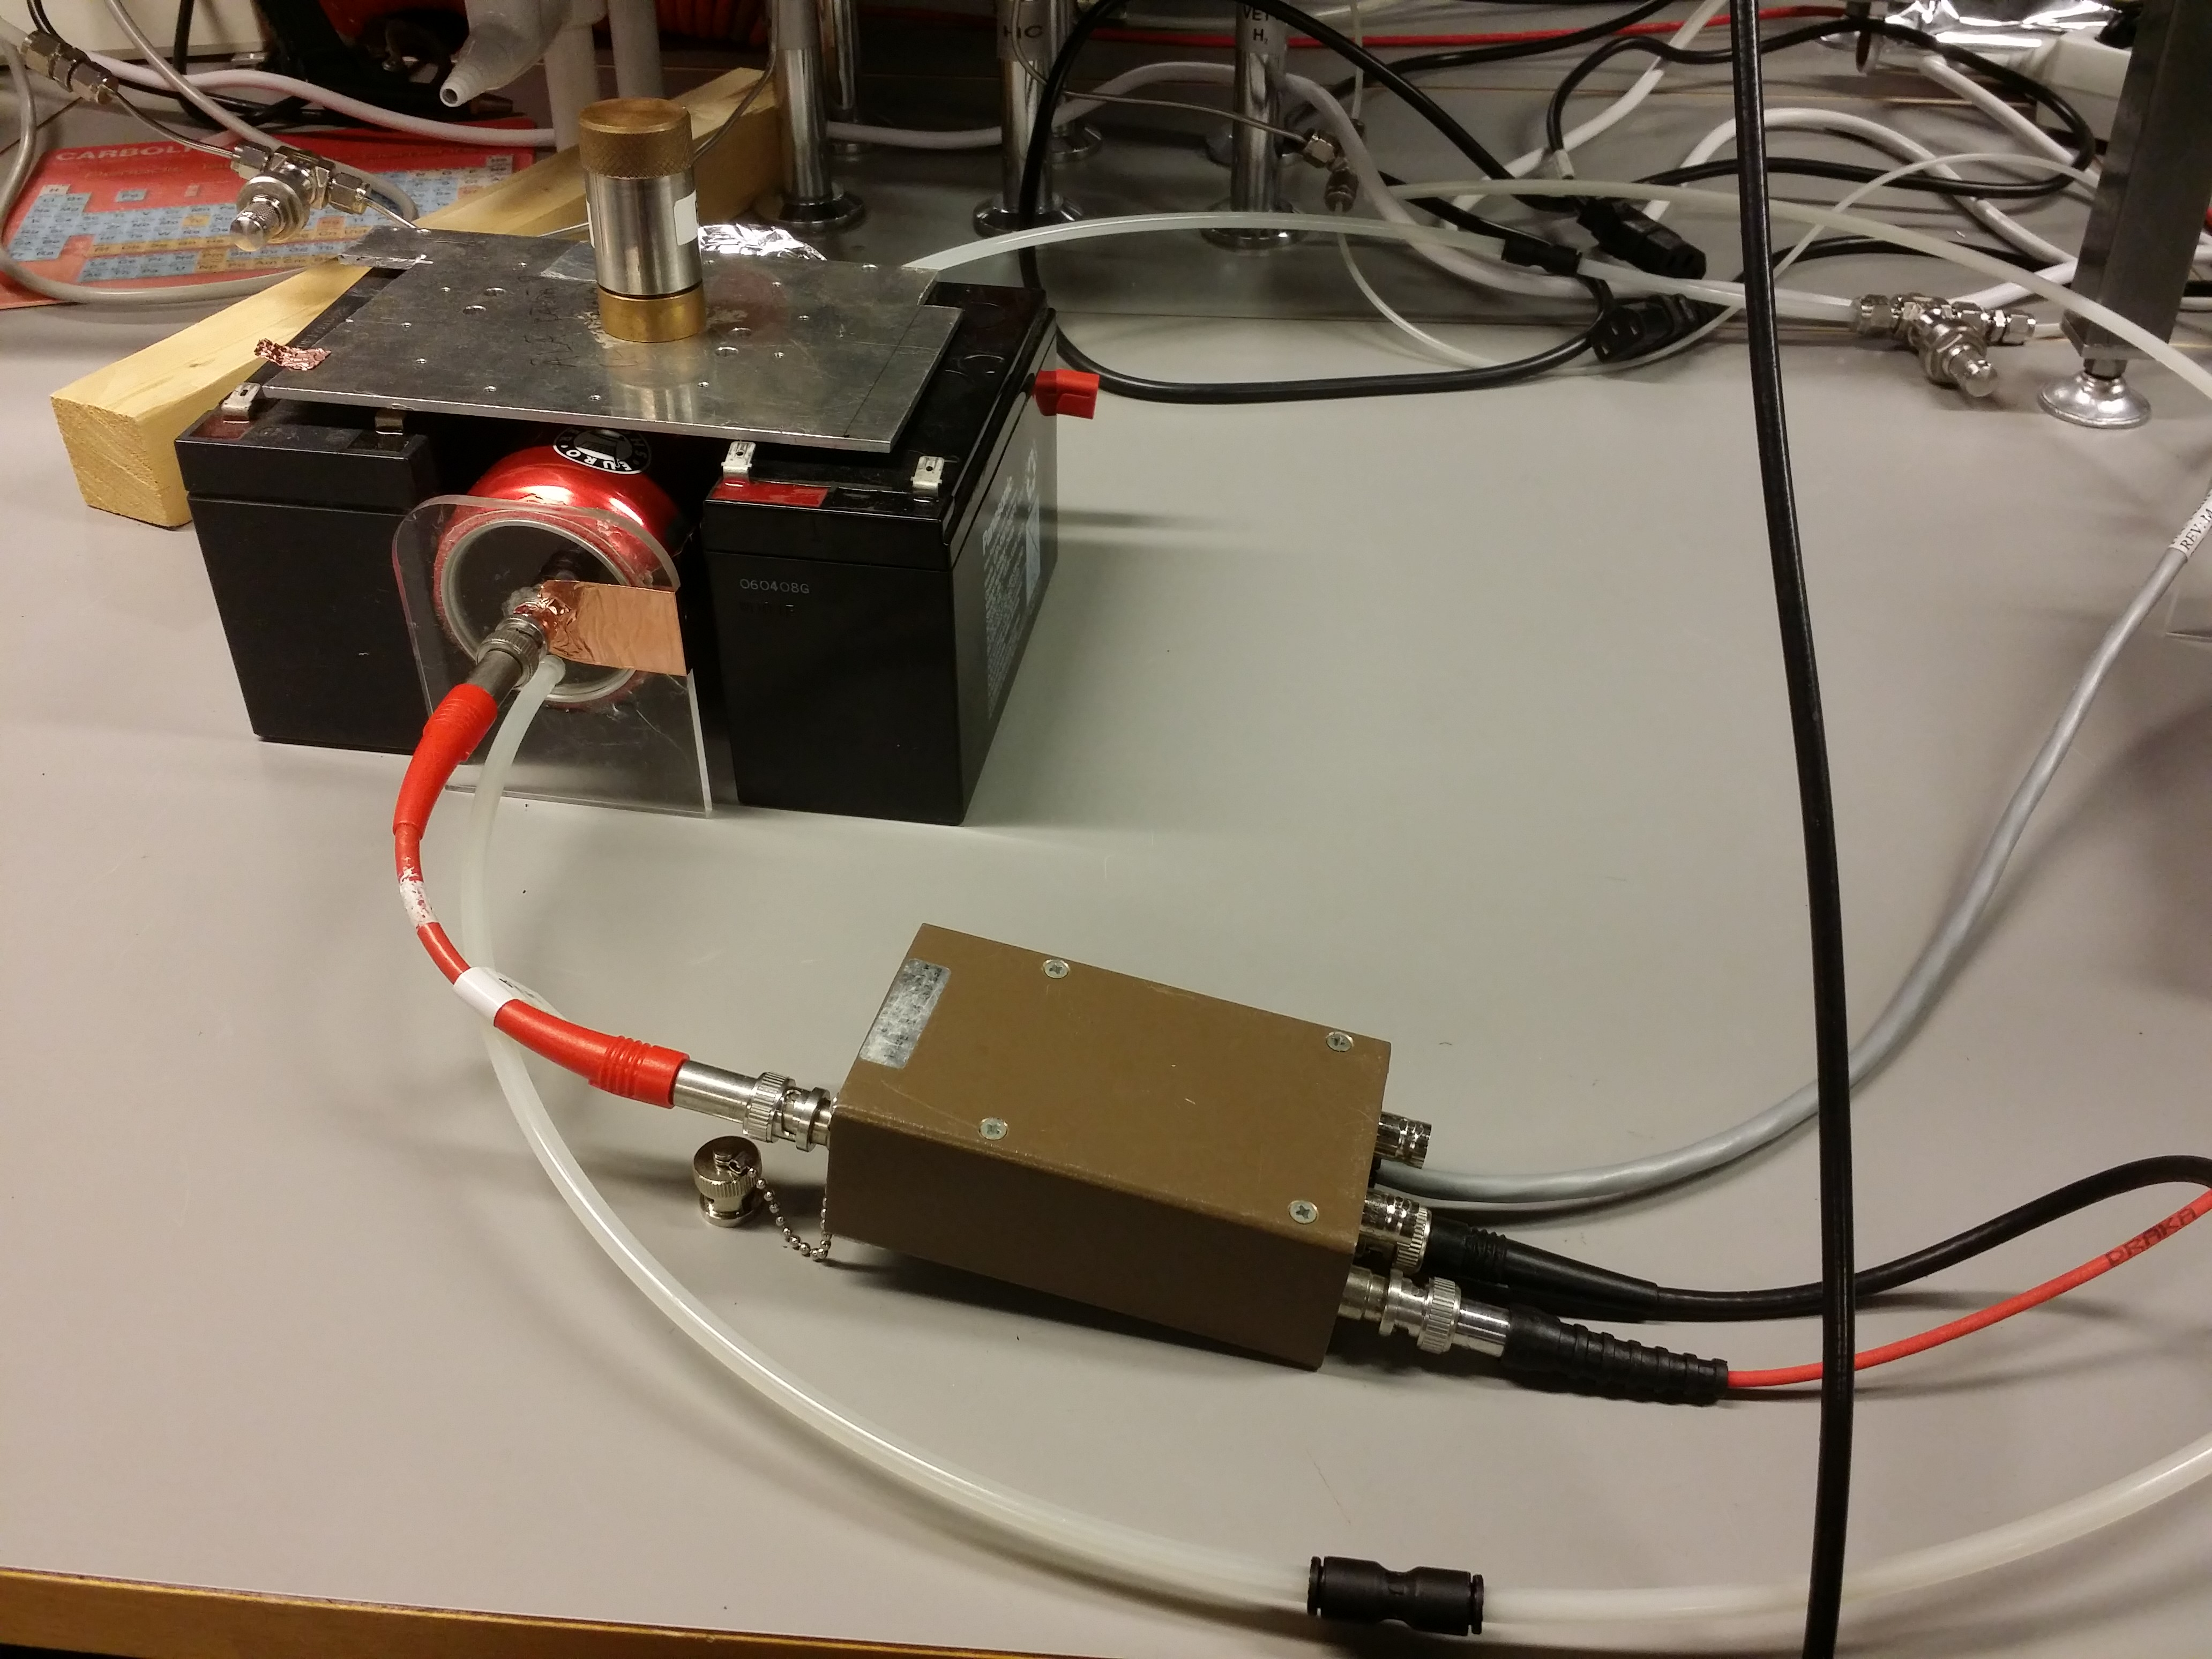
\includegraphics[width=\textwidth]{fig/IMG_20201130_144418.jpg}
\caption{Setup for testing with an Fe-55 source and a rack-mounted amplifier}
\end{figure}


\FloatBarrier
\section{Results and discussion}


\subsection{Calibration}
Output vs. input signal
See the spreadsheet!

\subsection{High voltage sweep}
The effect of gain settings and detector voltages

\subsection{Spectral measurement}
Some nice MCA spectra here
The uncertainty is not merely the width of the peak. We have to estimate all the uncertainties involved and propagate the errors.


\section{Conclusions}
Discuss results in context.
No need to repeat the results.
Refer to the introduction.
Was the aim fulfilled?
Were the results as expected? If not, why?
Is the mesurement precise enough to discuss ASDF?


\clearpage
\begin{appendices}

\section{Pre-amplifier}
\label{pre_amp}

Construction and detailed characterization here

\begin{figure}[ht!]
\centering
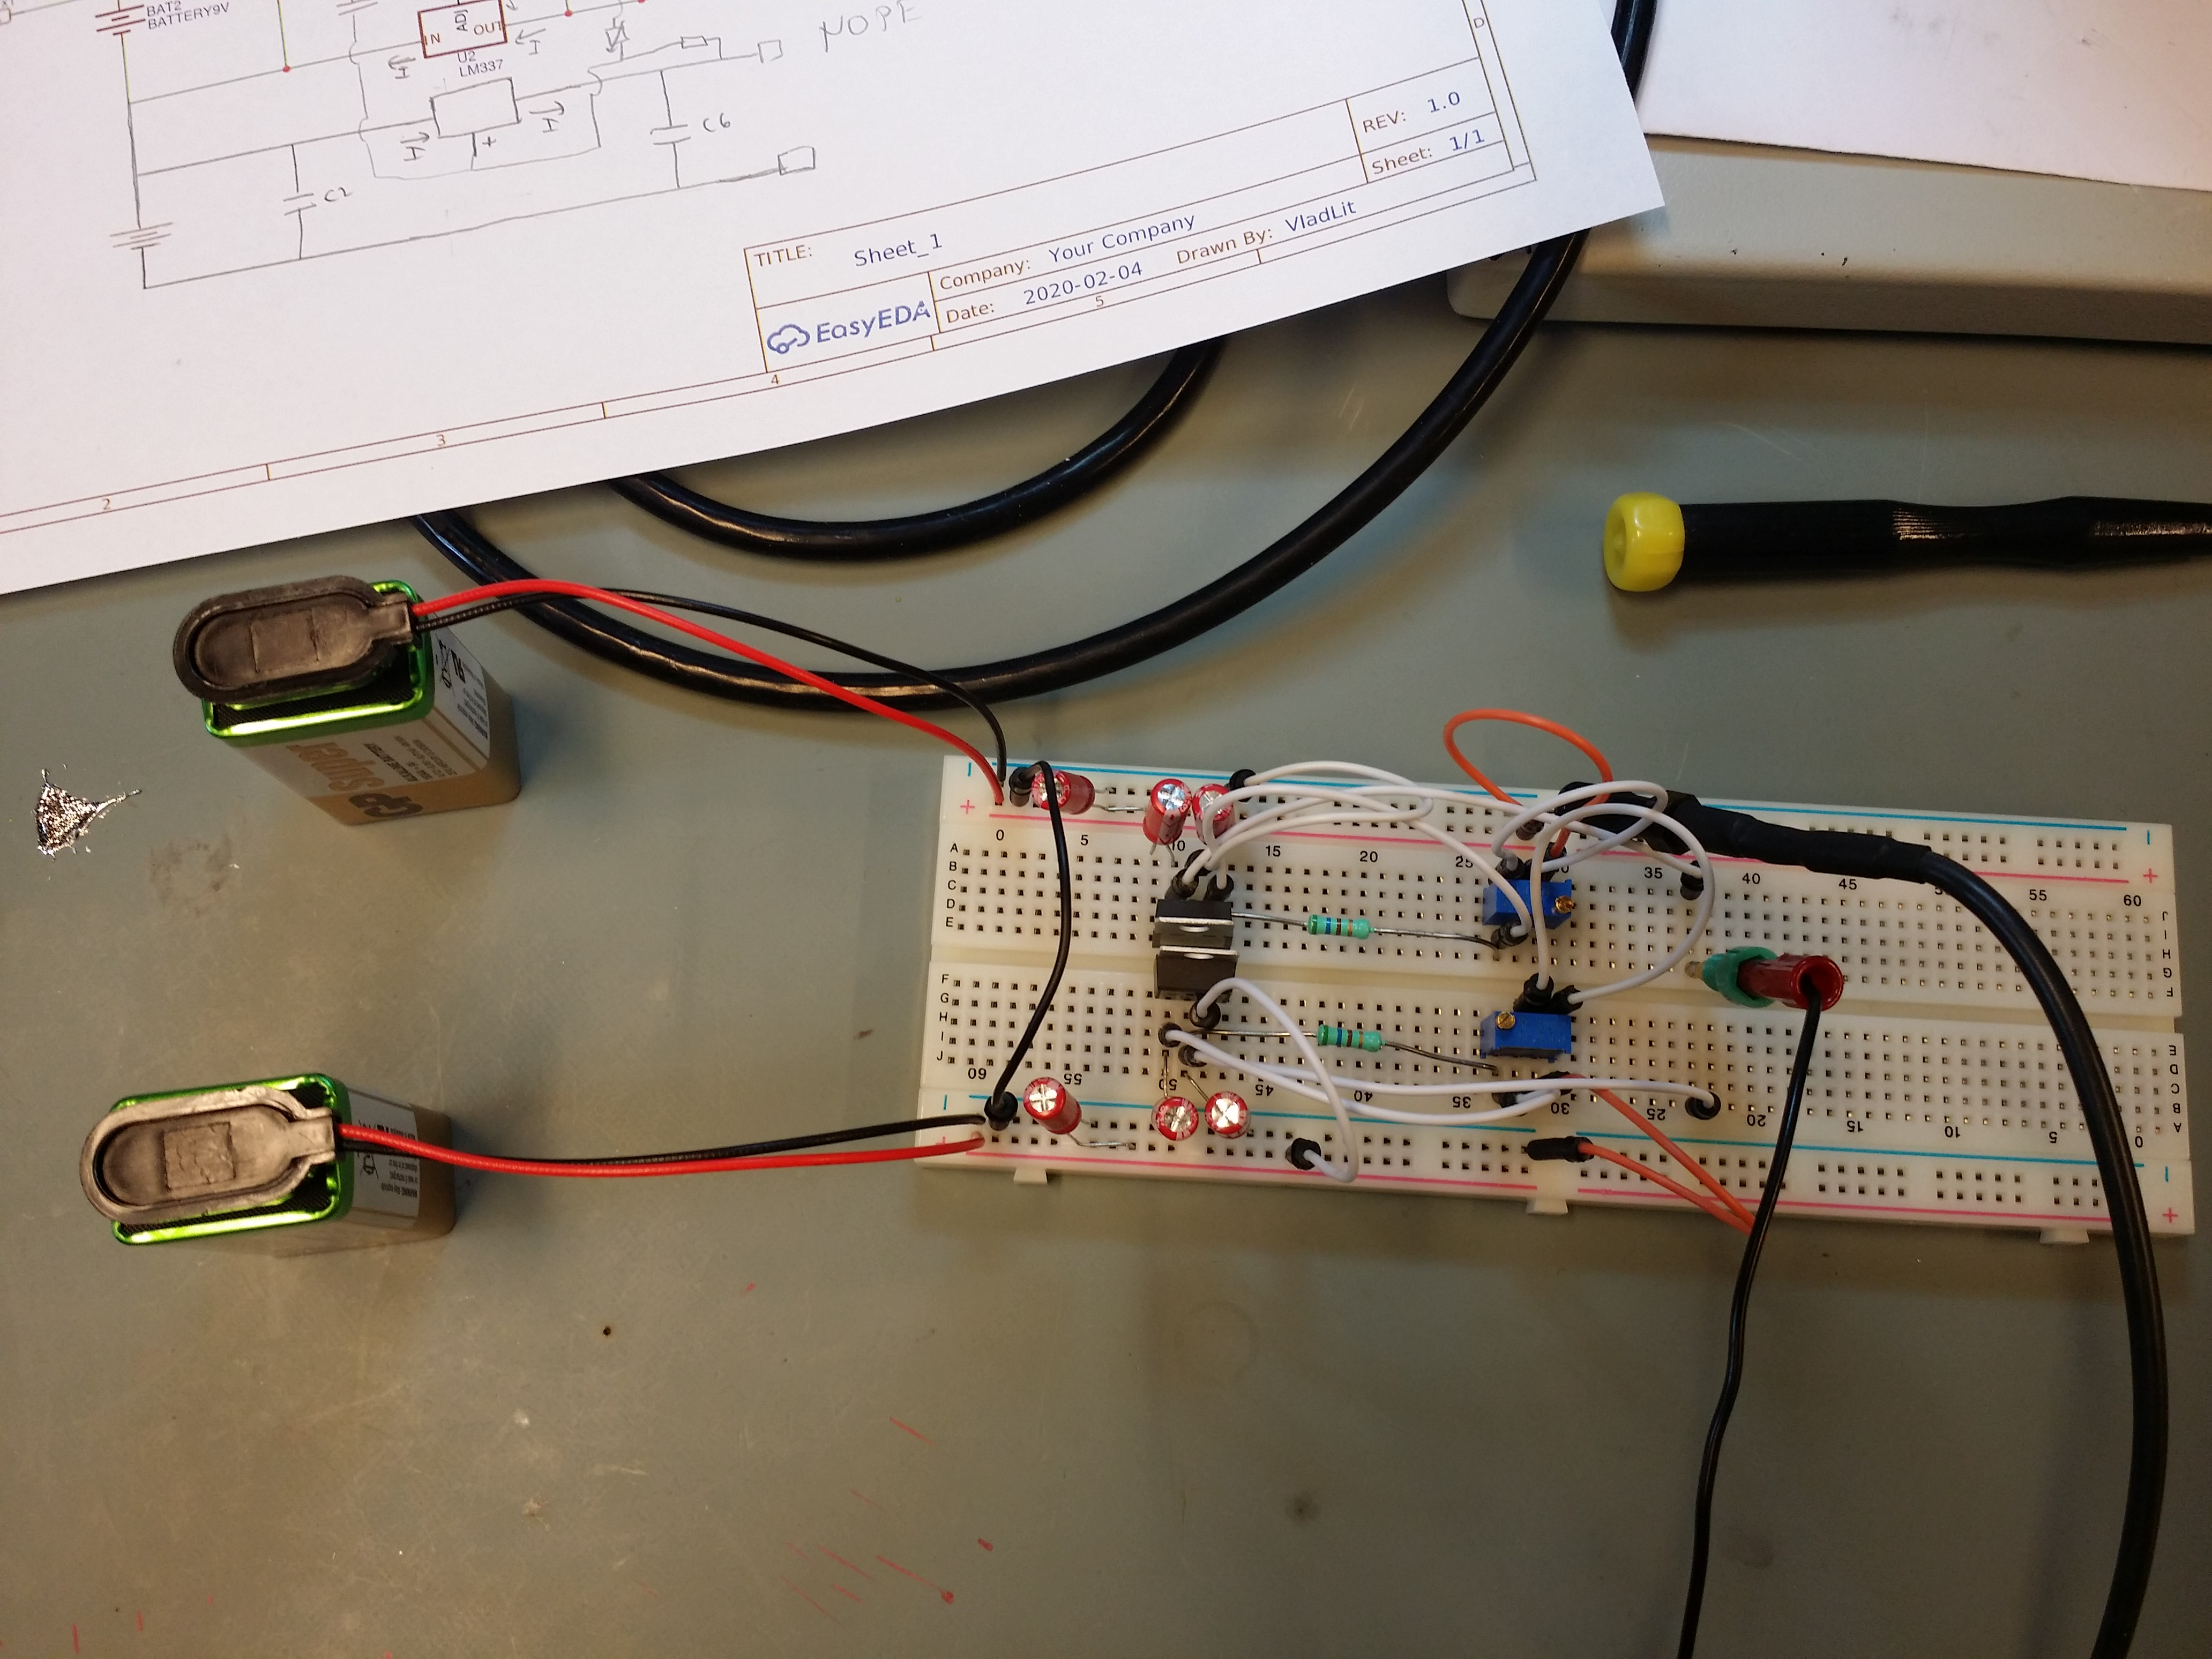
\includegraphics[width=\textwidth]{fig/IMG_20201005_104331.jpg}
\caption{Preliminary testing of the pre-amplifier components}
\end{figure}


\begin{figure}[ht!]
\centering
\subcaptionbox{}{
	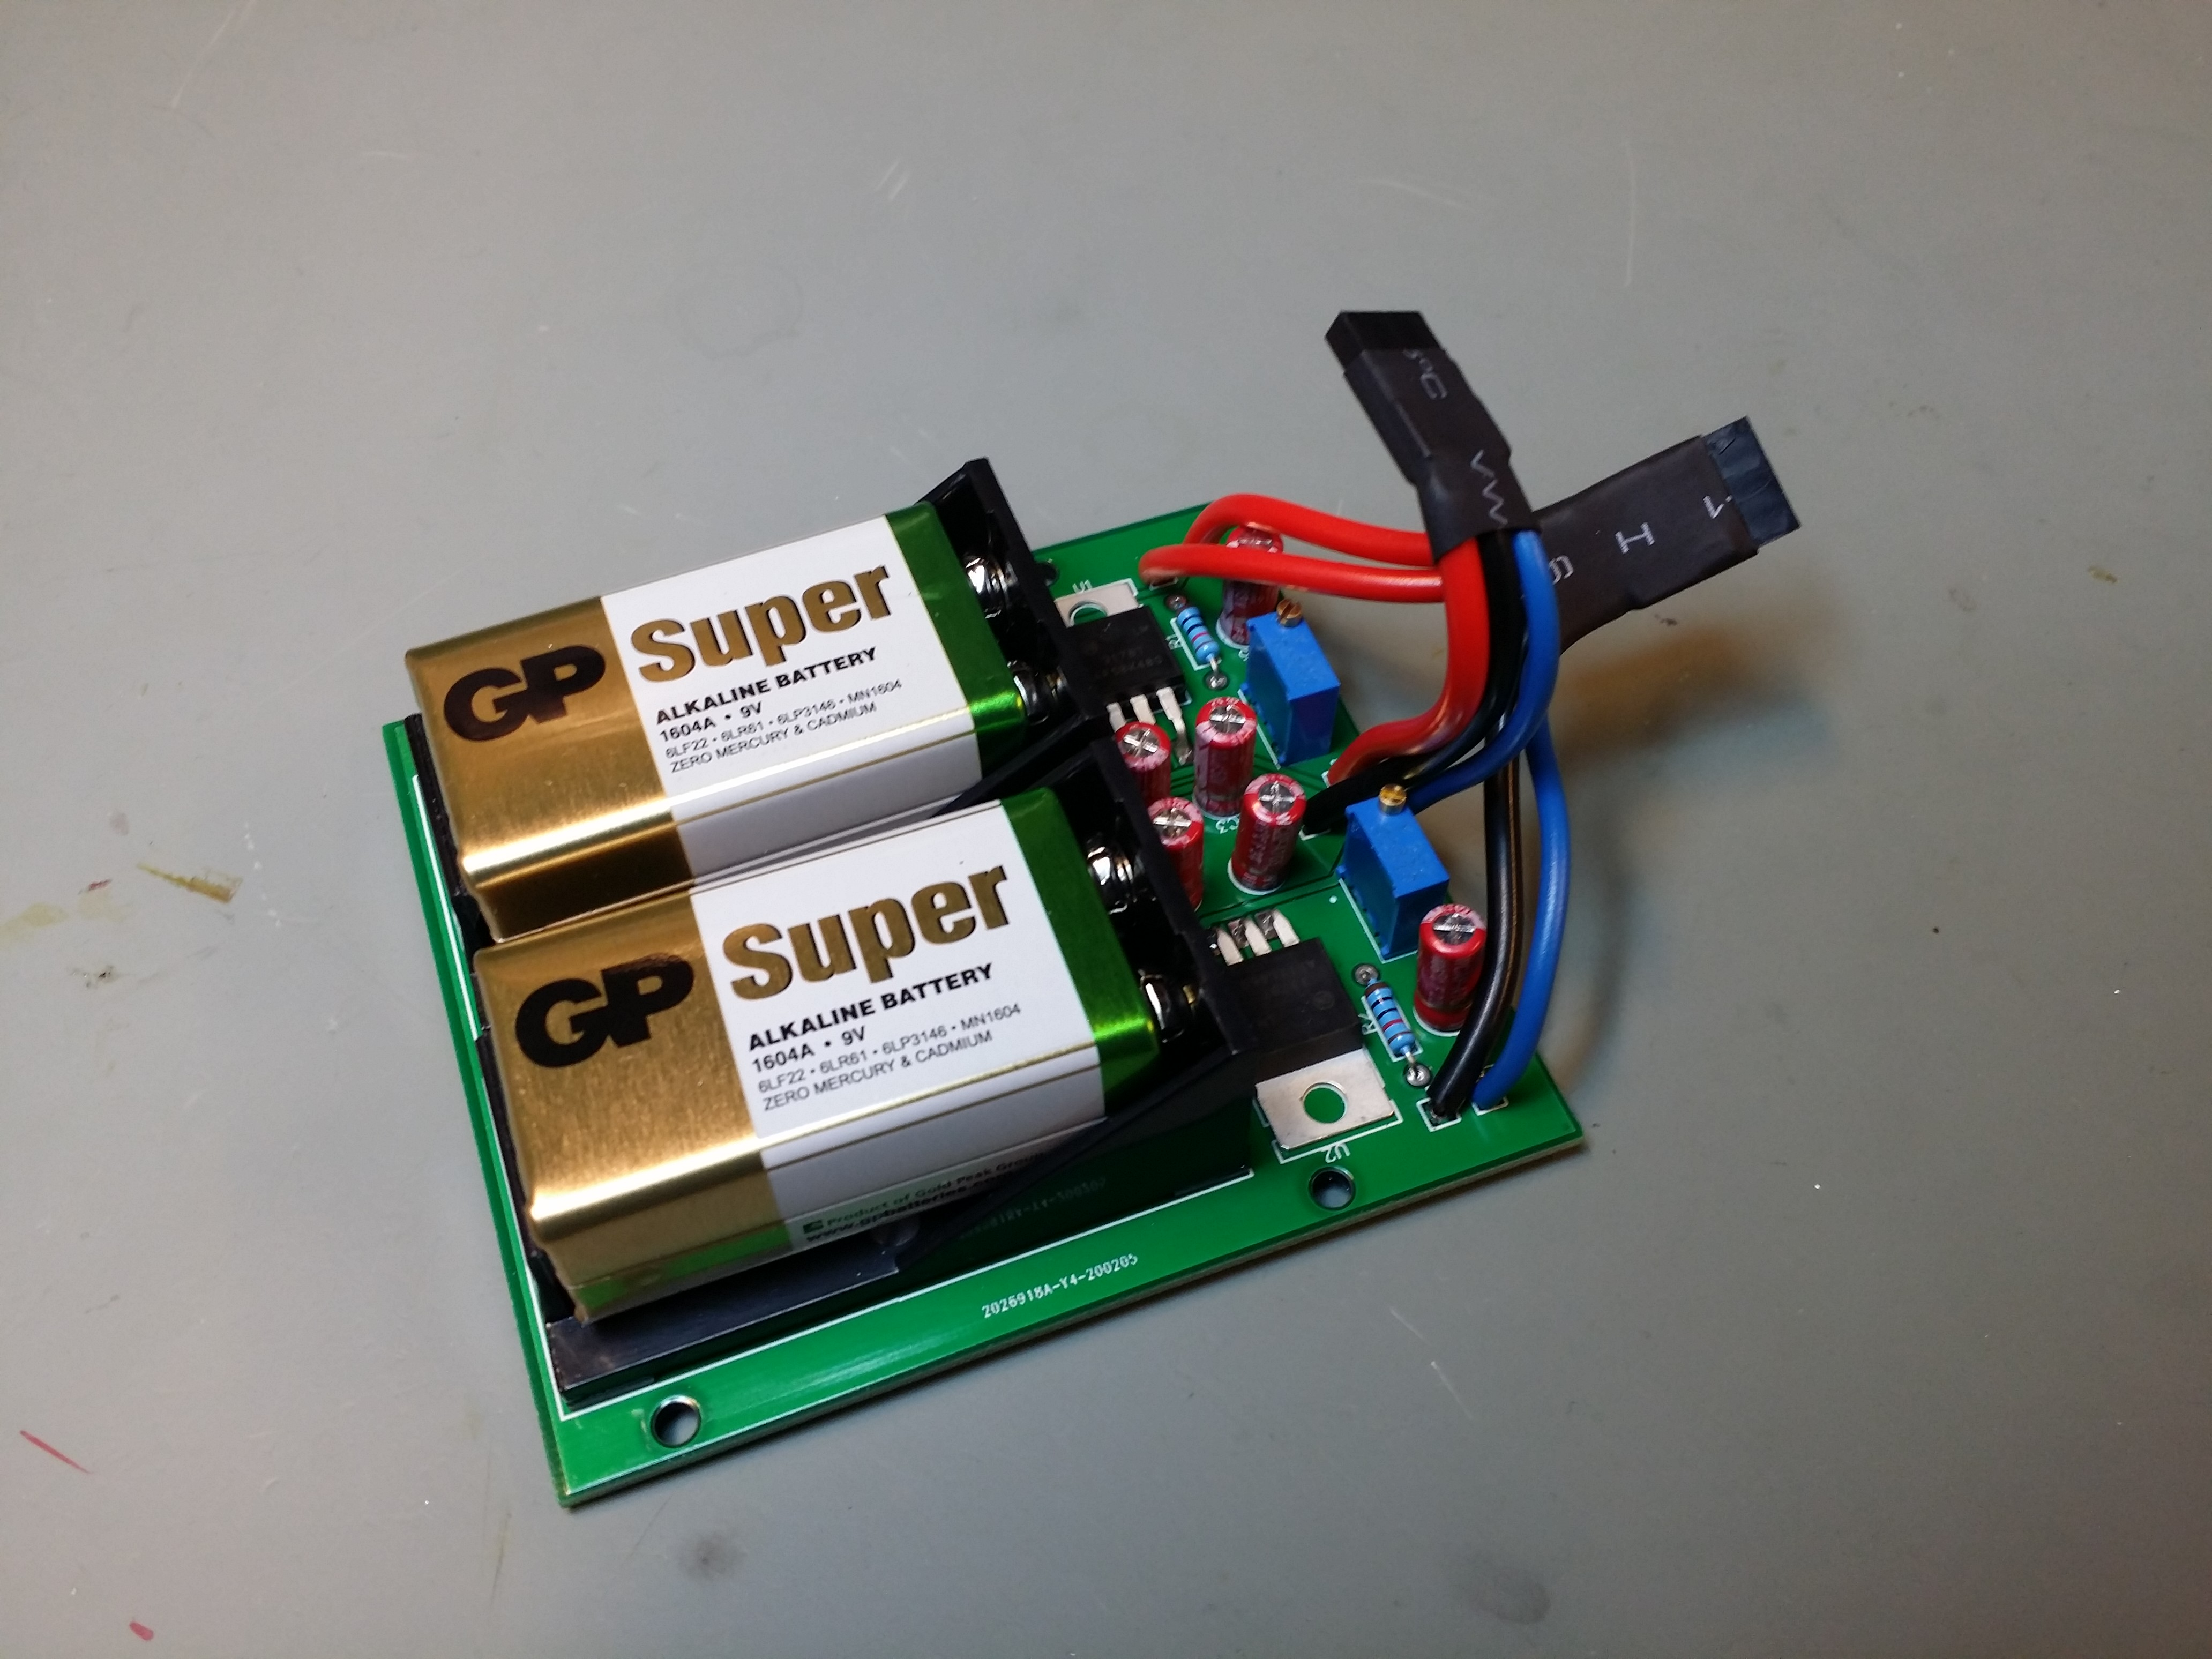
\includegraphics[width=\textwidth]{fig/IMG_20201201_121635.jpg}
}
\subcaptionbox{}{
	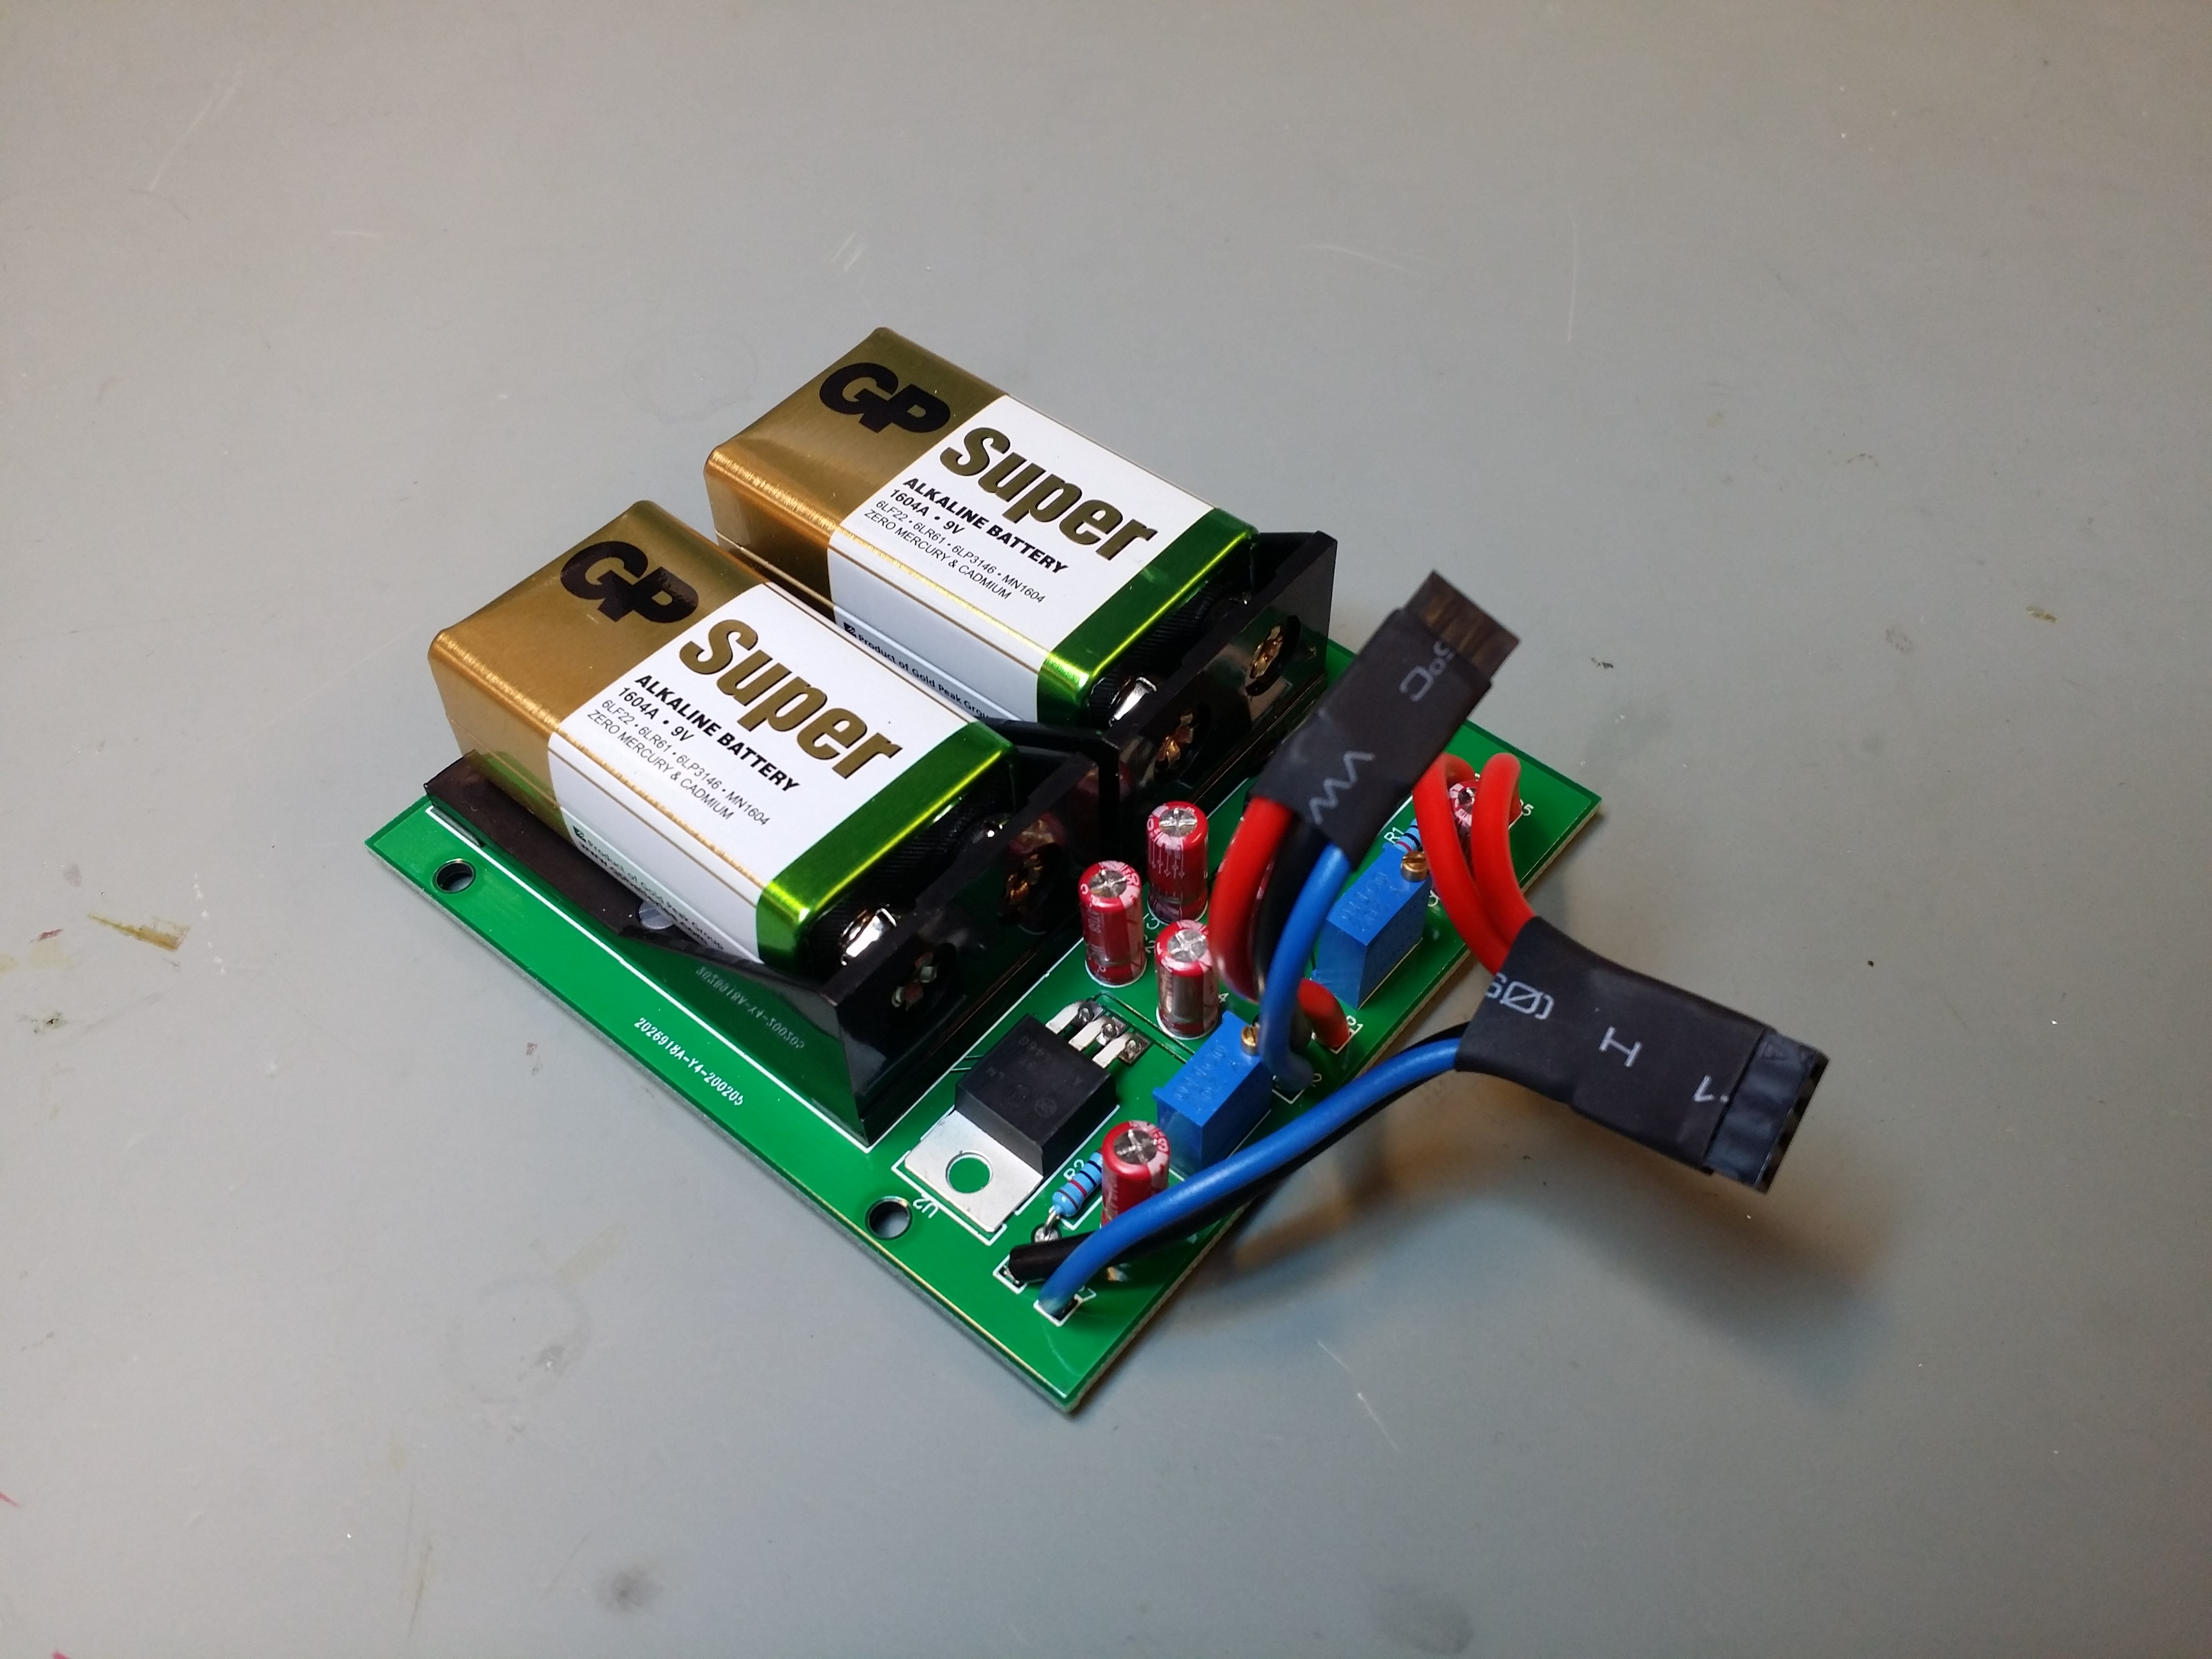
\includegraphics[width=\textwidth]{fig/IMG_20201201_121625.jpg}
}
\caption{Power supply for the pre-amplifier}
\end{figure}

\begin{figure}[ht!]
\centering
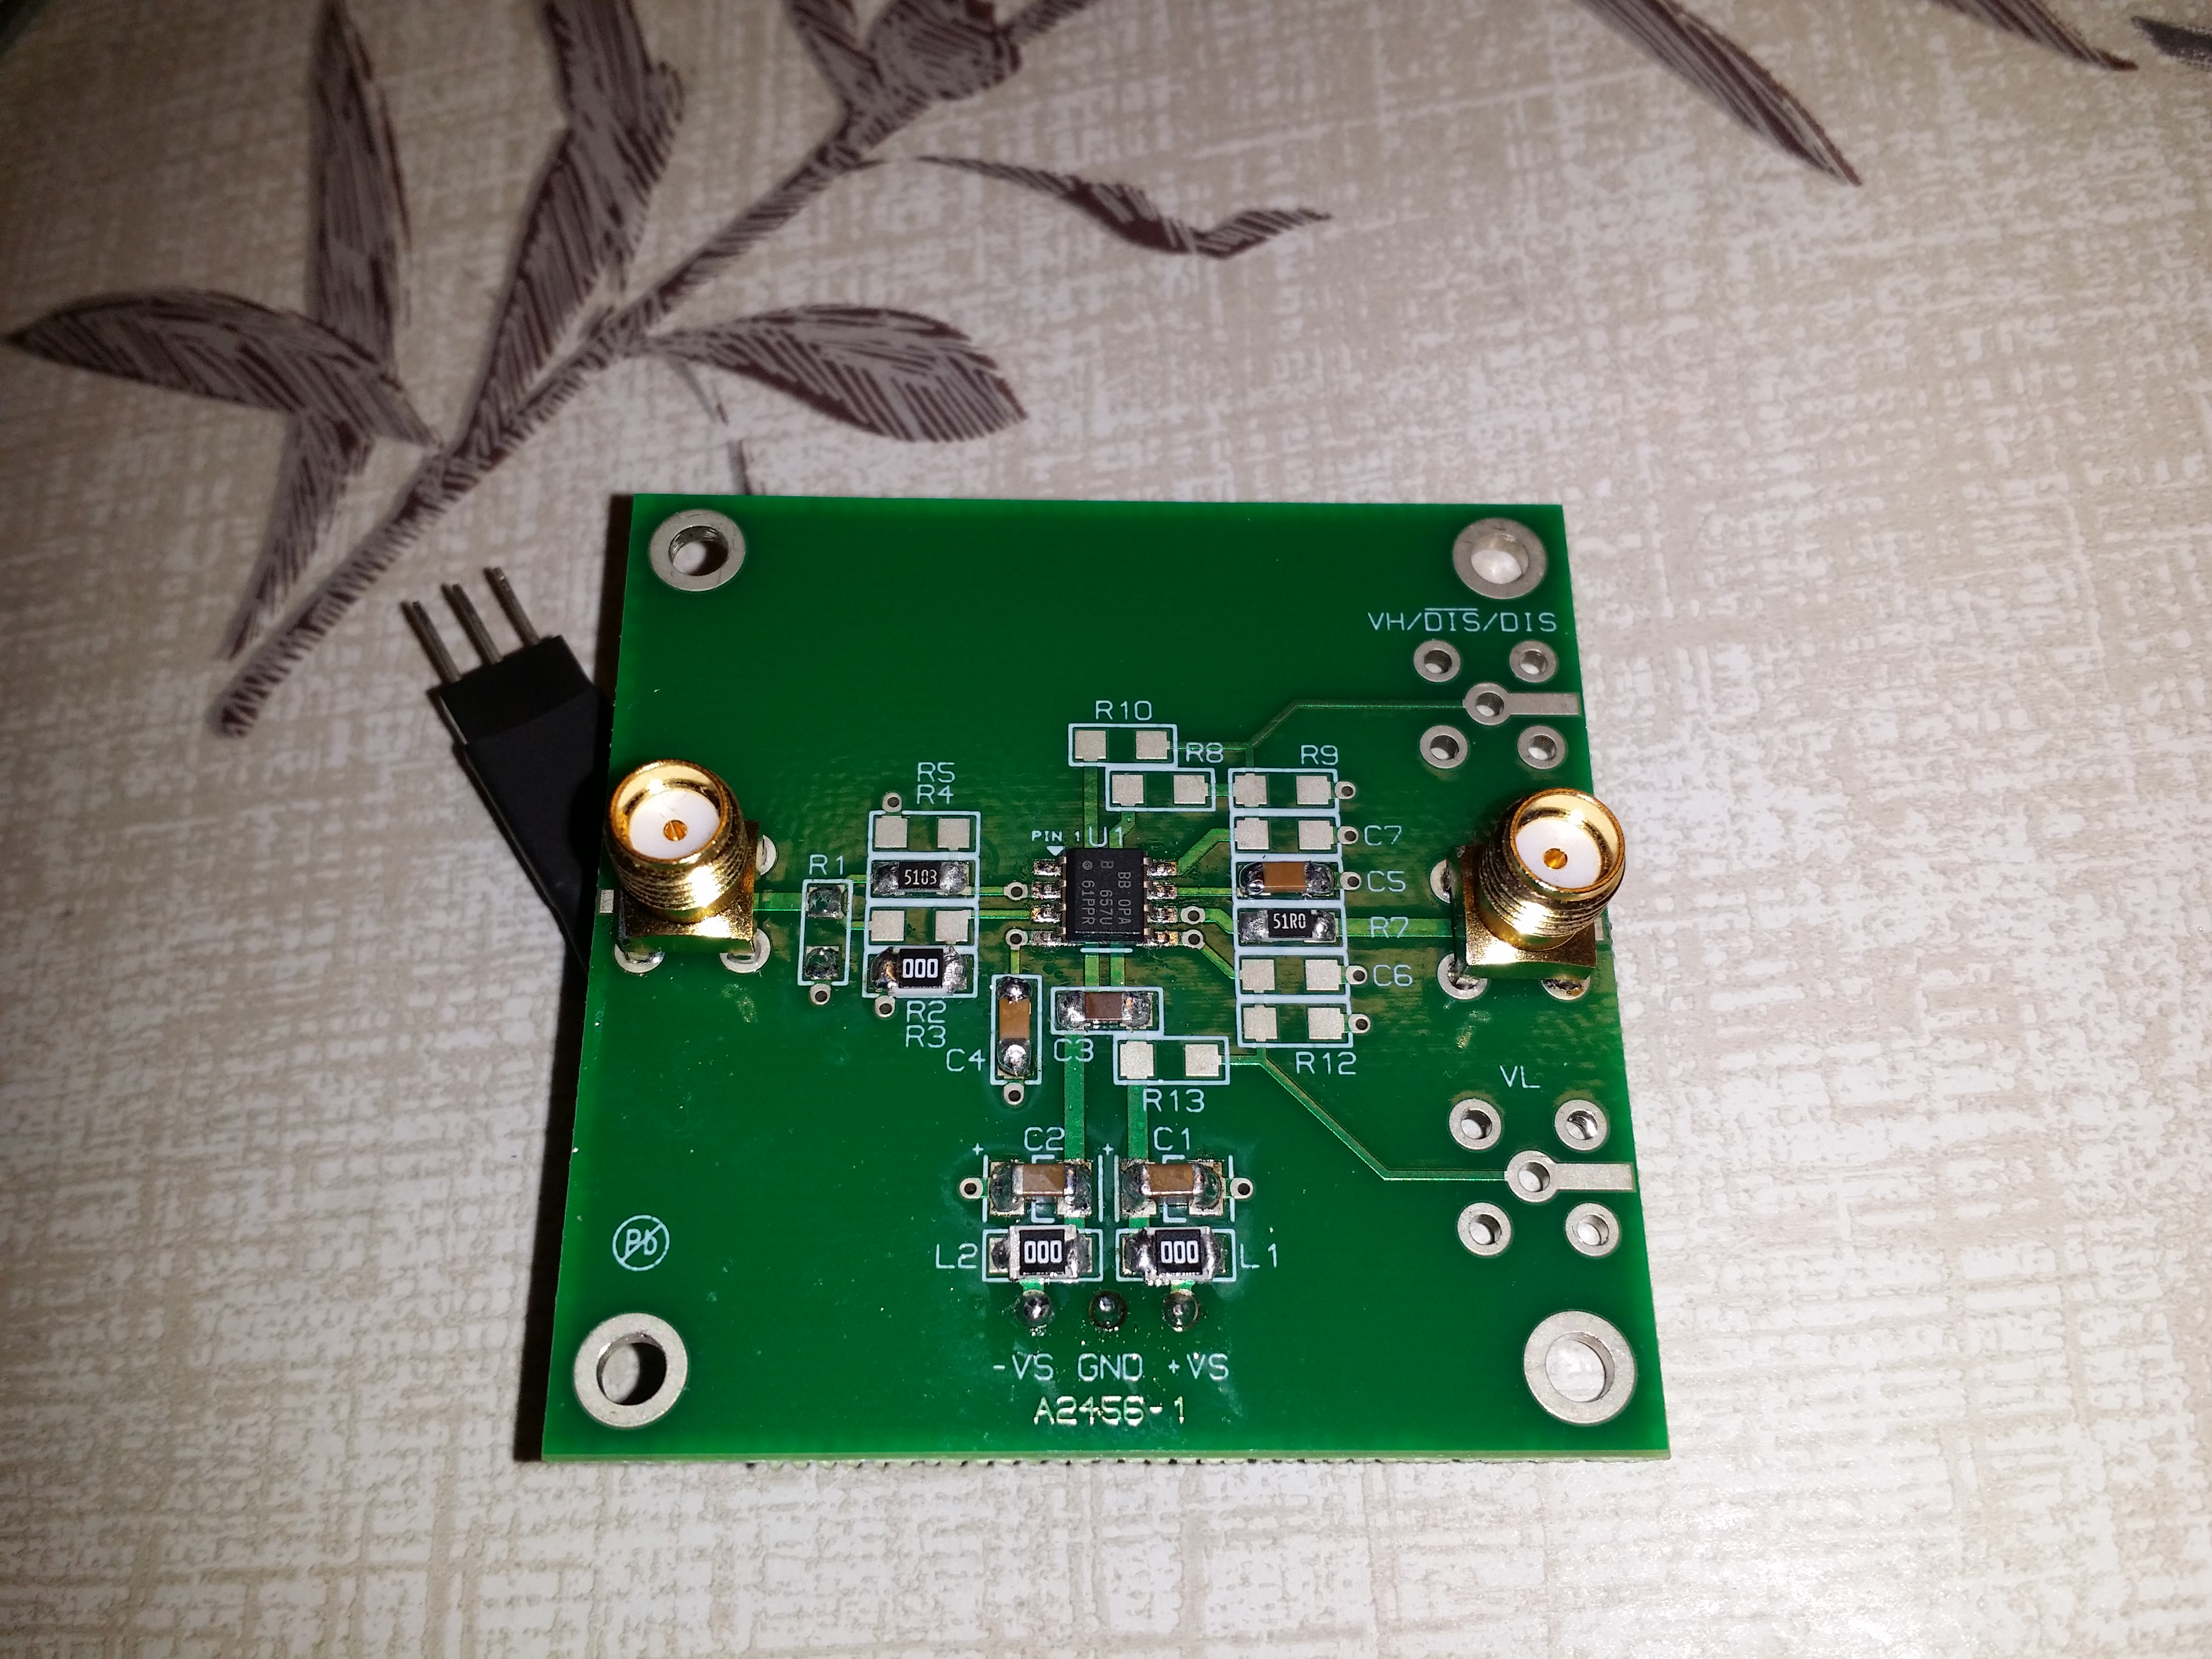
\includegraphics[width=\textwidth]{fig/IMG_20201207_121010.jpg}
\caption{Pre-amplifier board}
\end{figure}

\begin{figure}[ht!]
\centering
\subcaptionbox{}{
	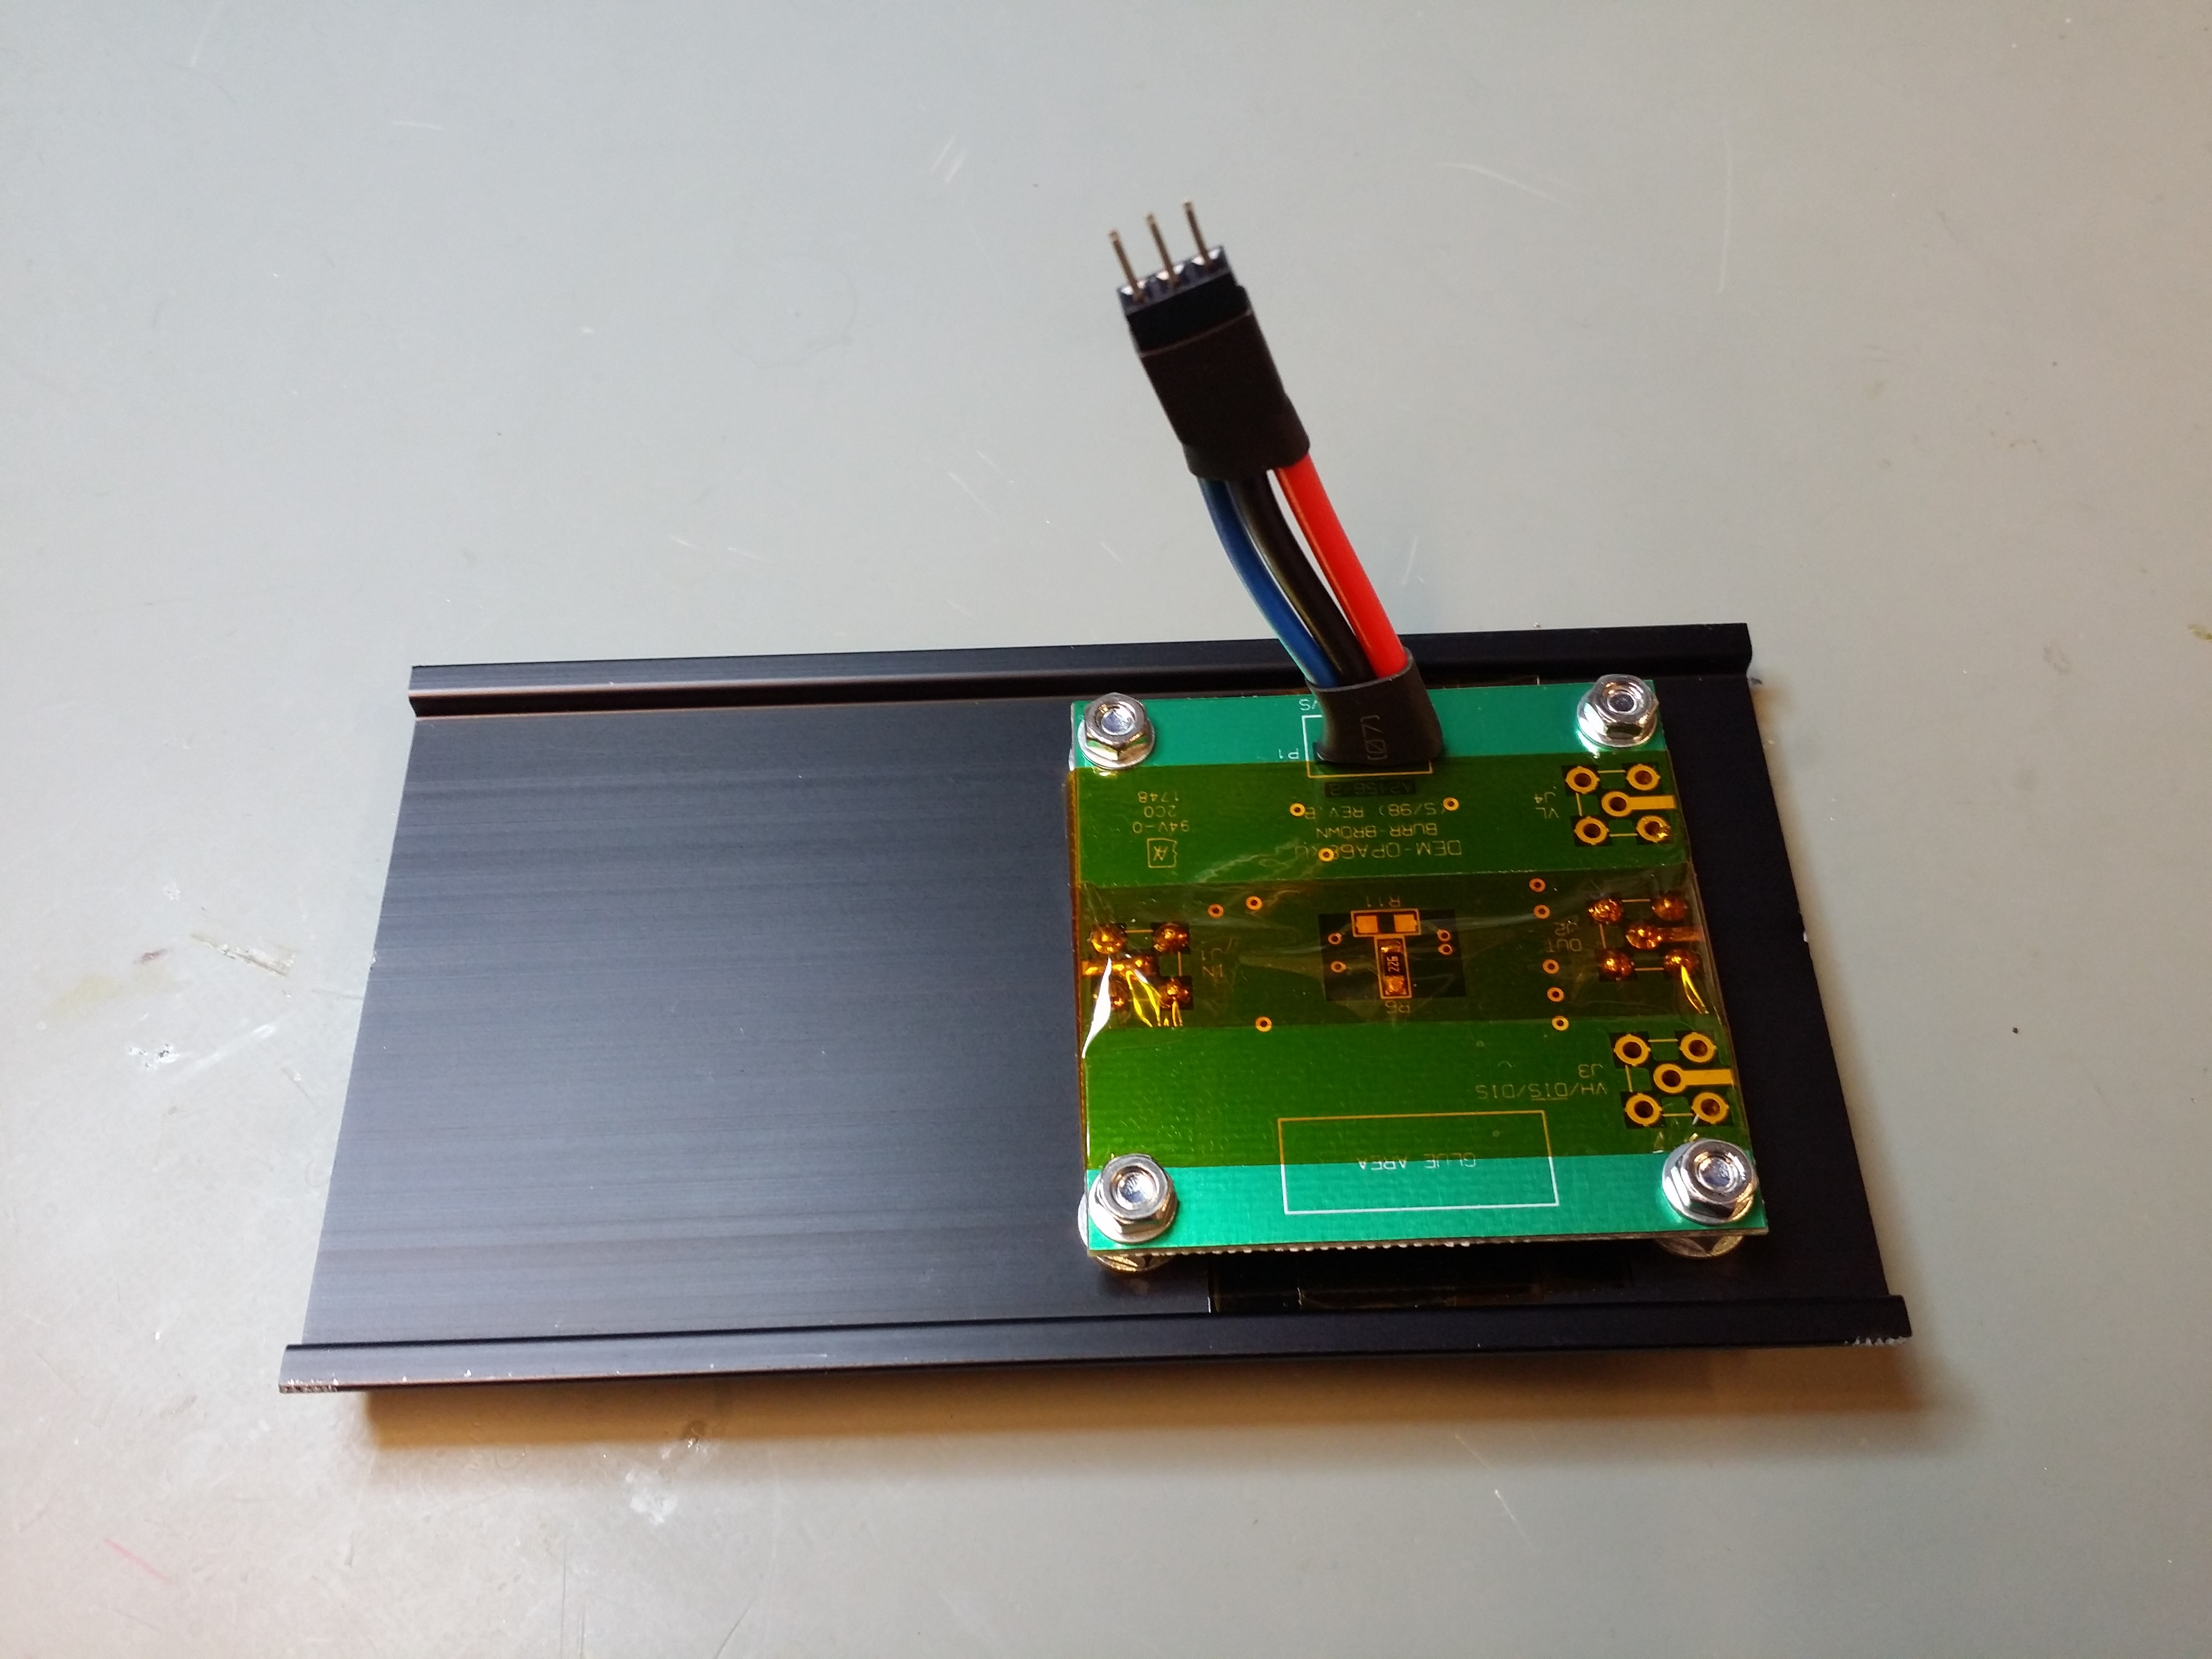
\includegraphics[width=\textwidth]{fig/IMG_20201201_121735.jpg}
}
\subcaptionbox{}{
	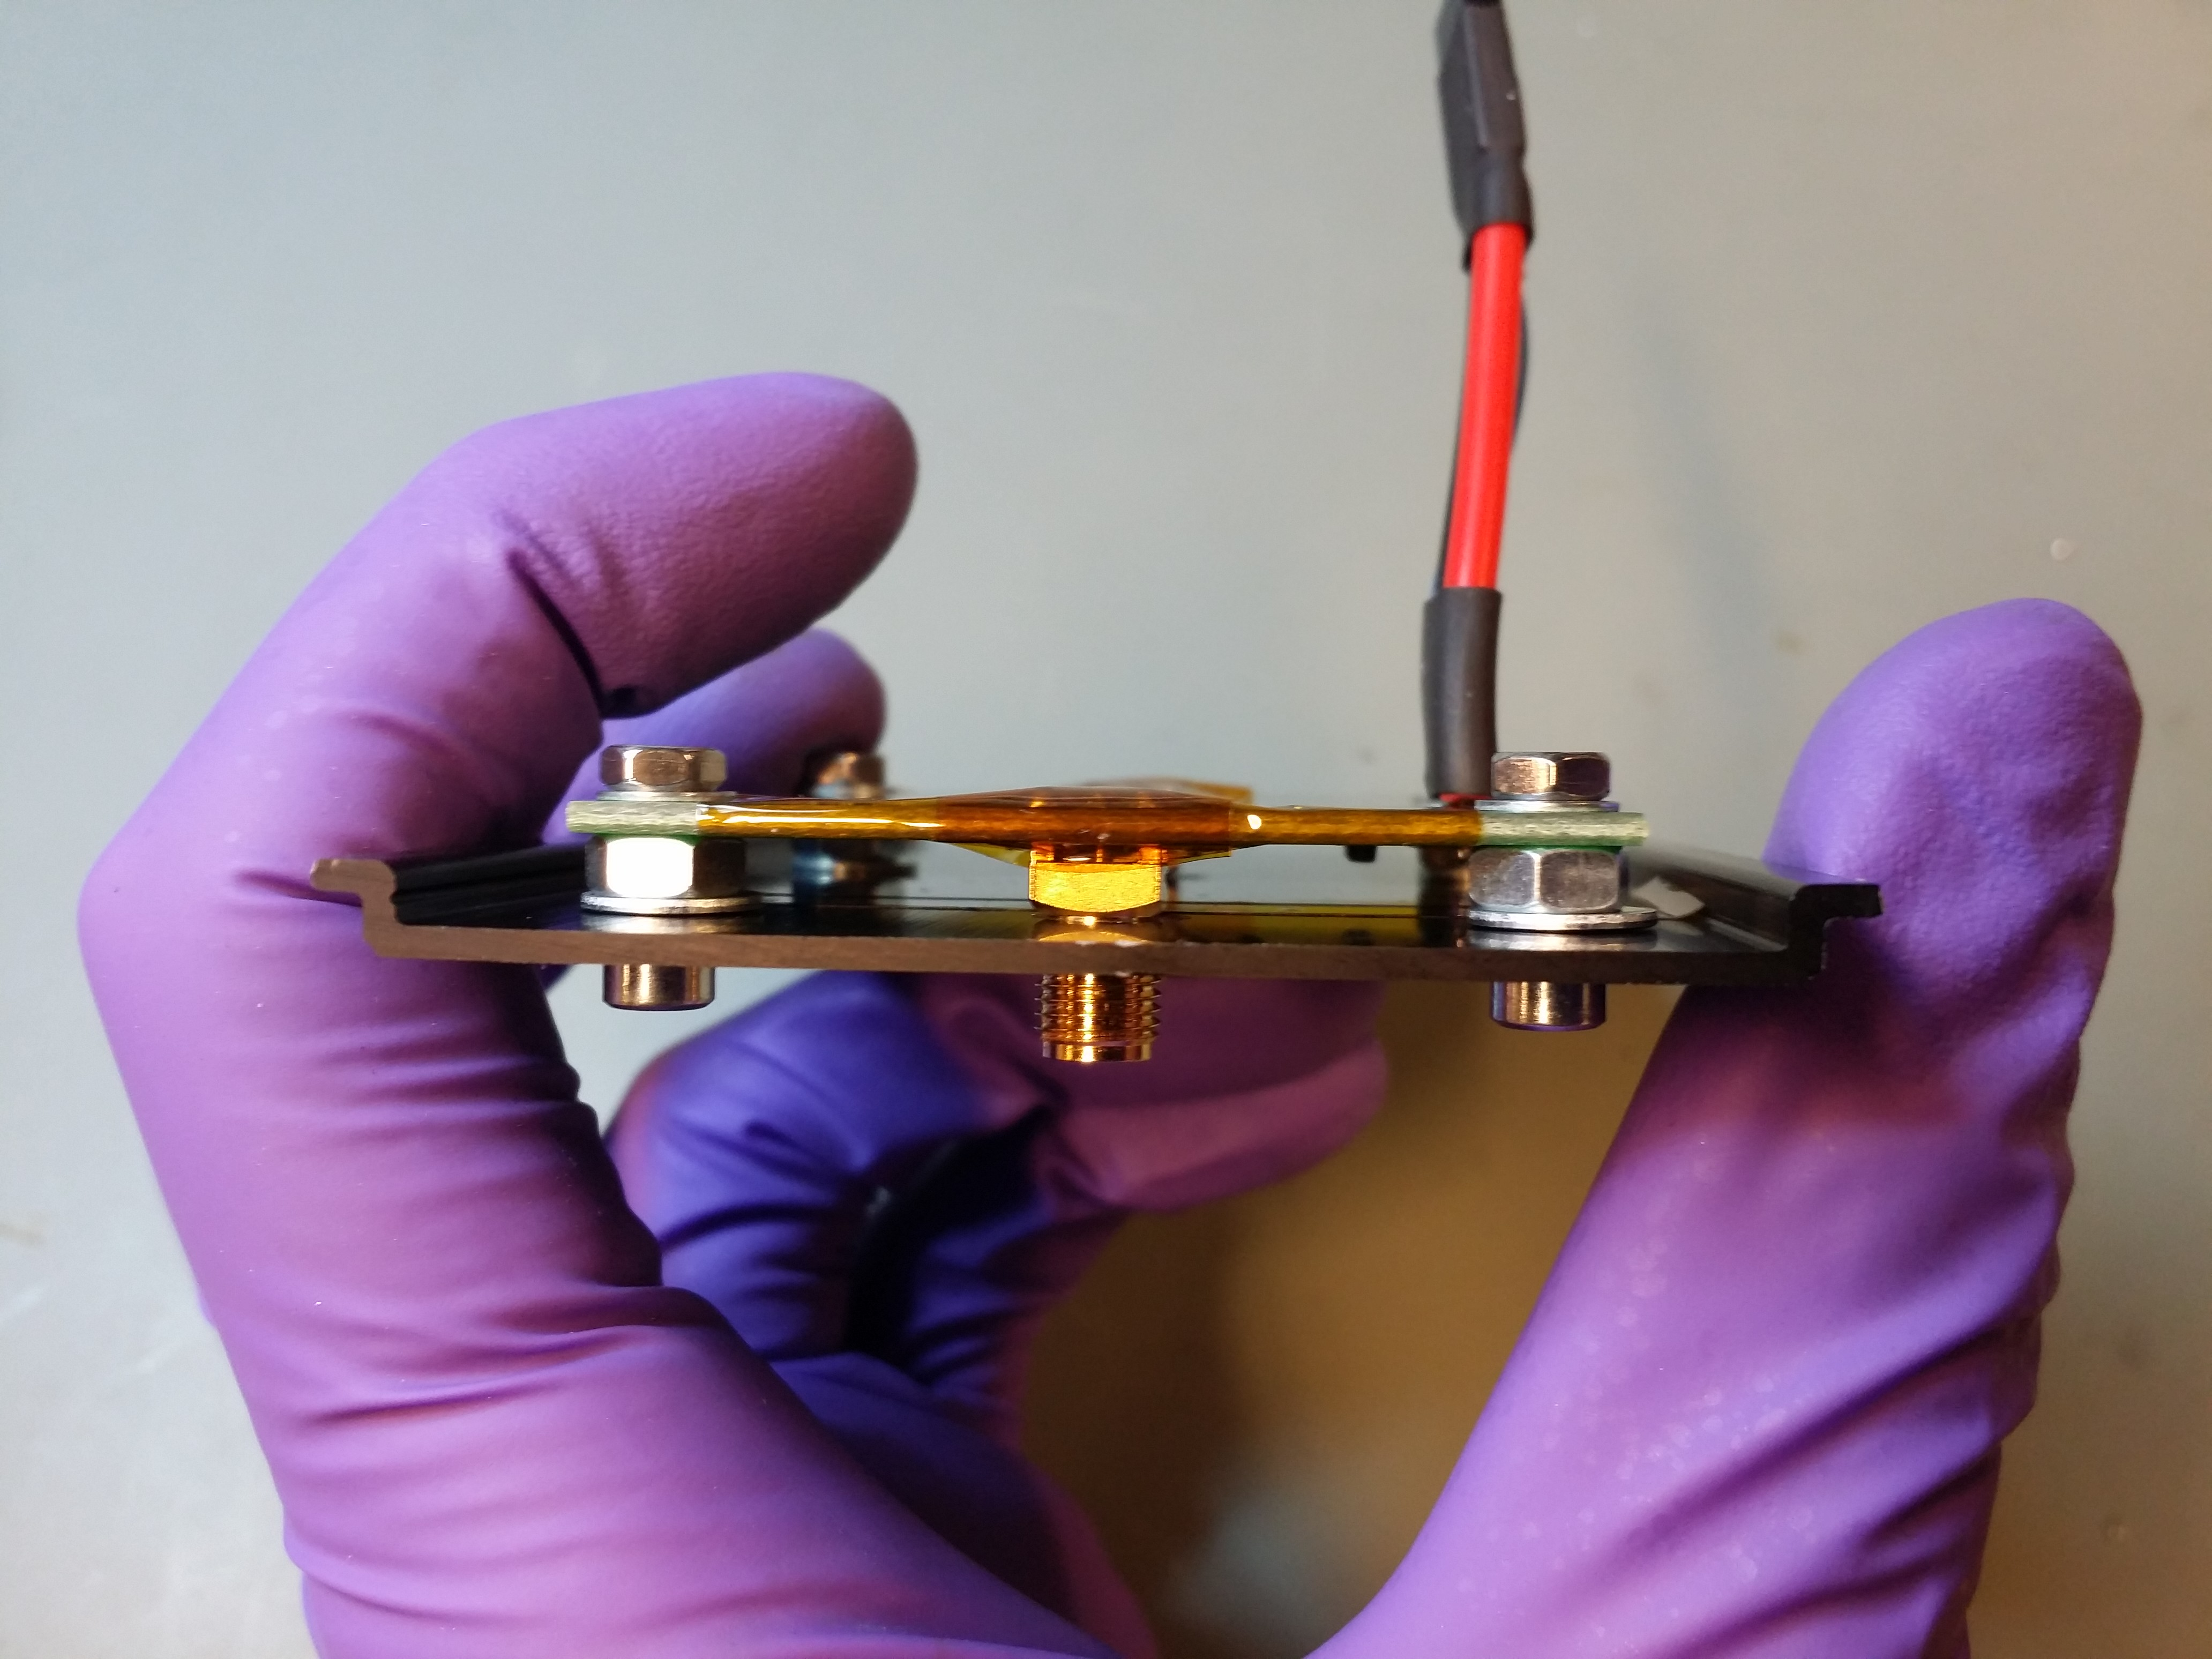
\includegraphics[width=\textwidth]{fig/IMG_20201201_121845.jpg}
}
\caption{Mounting of the pre-amplifier board}
\end{figure}

\end{appendices}


\clearpage
\section{References}
\printbibliography


\end{document}